%!TEX encoding = UTF-8 Unicode
%!TEX program = xelatex

\documentclass[bachelor]{ustcthesis}
% bachelor|master|doctor
\usepackage{ustcextra}
\graphicspath{{figures/}}
\bibliographystyle{ustcauthoryear}
% \bibliographystyle{ustcnumerical}

\renewpagestyle{front}[\zihao{-5}]{
    \sethead{}{软件工程作业管理系统概要设计}{}
    \setfoot{}{\thepage}{}
    \headrule
}
\renewpagestyle{main}[\zihao{-5}]{
    \sethead{}{软件工程作业管理系统概要设计}{}
    \setfoot{}{\thepage}{}
    \headrule
}
\newcommand{\HRule}{\rule{\linewidth}{0.5mm}}
\newcommand{\tabincell}[2]{\begin{tabular}{@{}#1@{}}#2\end{tabular}}

% RED information macro
\newcommand{\R}[1]{\textcolor{red}{#1}}

\begin{document}



\begin{titlepage}
\begin{center}
~\\[5cm]
\HRule \\[0.4cm]
{\huge \bfseries 四季云音乐 (音乐播放系统)\\概要设计}\\[0.4cm]
\HRule \\[1.5cm]

\begin{tabular}{ccc}
  & 人员 & 日期 \\ 
拟制 & 李嘉豪\ 鲁吴越\ 王若晖 & 2018-05-20 \\ 
评审人 & • & • \\ 
批准 & • & • \\ 
签发 & • & • \\ 
\end{tabular} 

\end{center}
\end{titlepage}



\frontmatter
\begin{abstract}
本文是软件工程需求规格说明书模板,修改自于中国科学技术大学本硕博毕业论文 \LaTeX{} 模板示例文件,该模板由
zepinglee和seisman创建,遵循中国科学技术大学的论文写作规范,适用于撰写学士、硕士和博士学位论文。

本文档最后一章演示如何使用 \LaTeX{} 的一些基本命令以及本模板提供的一些特殊功能,
模板的选项及详细用法请参考模板说明文档 ustcthesis.pdf。请在提交之前把最后一掌实例注释掉。

\keywords{软件工程\zhspace{} 中国科学技术大学\zhspace{} 学位论文\zhspace{} \LaTeX{}~通用模板\zhspace{} 学士\zhspace{}
硕士\zhspace{} 博士\zhspace{} 示例文档\zhspace{} 模板说明文档}

\begin{table}[htbp]
\centering
\caption{缩略词清单} \label{tab:abbr}
\begin{tabular}{|c|c|c|}
    \hline
    缩略语 & 英文全名 & 中文解释 \\
    \hline
    c & d & e\\
    \hline
\end{tabular}
\end{table}

\end{abstract}

\tableofcontents
\listoffigures
\listoftables
% \listofalgorithms  % 算法索引,如不需要,可直接注释掉本行
% \begin{notation}

%\centering
%XX 软件需求规格说明书

%关键词:能够体现文档描述内容主要方面的词汇。
 
%摘要:


\centering
\begin{tabular}{rl}
$\ln x$ & natural logarithm $\log_ex$ \\
$\log x$ & common logarithm $\log_{10}x$ \\
$x\ \mathrm{mod}\ y$ & remainder \\
\end{tabular}

\end{notation}


\mainmatter
\chapter{简介}
\section{目的}
This section should state the purpose of the document. It could also specify the intended audience. Identify the product whose software requirements are specified in this document.

这部分要描述文档的目的。应该指明读者。说明本需求文档描述了哪个产品的软件需求。

\section{范围}
This section should address areas which this document includes and that are specifically excludes. 

本节应描述文档所包括和不包括的内容。

\chapter{总体概述}

\section{软件概述}
\subsection{项目介绍}

音乐使人们生活中不可或缺的一部分,
    而市面上,已经有许多成熟的音乐播放系统,
    为了达到产品生存与盈利,我们需要不同点与亮点。
我们的\proname 项目有两大竞争优势。

首先,本项目借助云服务器,达到用户“一次购买,随时随地,想听就听”,
    只要用户购买了歌曲,或者订阅了会员服务,
    就可以在任何时间、任何地点方便地收听到他有权限访问的歌曲。
为了达到这一点,我们需要强大的云服务器作为后端,
    并使得用户的购买记录能够安全、永久地被存储,
    并且,为了让用户能够尽可能在任何情况下收听到他购买的歌曲,
    我们需要为各种浏览器环境优化网页环境,
    并且在各种个人电脑系统上推出客户端,
    同时,各品牌、各平台、各系统的移动客户端也要跟上
    当今移动设备快速的迭代速度。

其次,我们的个性推荐服务能够让用户体验到“\proname 比你更懂你想听什么”
    的感受。
    我们需要建立用户大数据模型,根据用户的试听、购买、订阅行为,
    为用户加上各种标签,通过适配标签集与歌曲集之间的相关性,
    精确地将用户喜爱的歌曲推荐给用户。
这既可以增加用户粘度,又可以使用户受到推荐之后,购买更多的歌曲。

\subsection{产品环境介绍}

\begin{itemize}
    \item 我们的项目分为服务端与客户端,其中,服务端是统一的,
    所有客户端都由该统一服务端进行数据交互与信息支持;
    而为了满足用户多种多样的收听音乐的环境,
    我们的客户端有较多种类,
    目前,我们需要考虑以下客户端环境:
    \begin{enumerate}
        \item 网页浏览器环境,对应网页客户端;
        \item Windows环境,对应传统程序客户端和较新的
        Universal Application(应用商店内应用程序);
        \item Mac OS环境,对应一般程序客户端;
        \item Linux环境,对应一般客户端以及基于命令行的最小化客户端;
        \item iOS移动环境,对应iOS应用(App Store内应用程序);
        \item Android移动环境,对应安卓应用程序;
        \item 车载娱乐系统环境,对应厂商预装车载娱乐系统内程序;
        \item 电视机机顶盒环境,对应电视服务商提供的机顶盒内程序;
    \end{enumerate}
    \item
    \item
\end{itemize}

% 描述的是本产品与其它产品或项目所组成的整体环境。

% 1.如果本产品是独立的并完全自我包含,在此说明这一点。

% 2.如果SRS定义的产品是更大的系统或项目的组件(此种情形经常发生),那么应:

% 	A. 描述此大系统或项目每个组件的功能,并且标识接口。

% 	B.  确定本软件产品主要外部接口。( 注意:在此部分并不进行这些接口的详细描述;对这些接口的详细描述在SRS的其它 部分提供。)

%     C. 描述相关产品硬件和所使用的外部设备。(  注意:  这只是概述性描述。)

% 通过方块图来描述大系统或项目的主要组件,互连性以及外部接口将是非常有帮助的。本部分不应提出一个具体的设计解决方案或对解决方案的具体设计约束(具体设计约束将在具体需求章节中描述)。本部分内容是产生设计约束的基础。

\section{软件功能}
Summarizes the major functions that must be implemented through the software, and the functions to be implemented through user operation. Details will be provided in the Specific Requirement, so only a summary (such as a directory list) is needed here. The functions should be organized to make them understandable to the readers, and be appropriate for subsequent design and tests. Diagrams like top-level data flow diagram or object class diagram are recommended to illustrate the relationships among the major requirement groups

Sometimes, this section can directly refer to the superior specification of the software that allocate the specific requirements to this software ( if existed ).
The specific requirements should not be described in this section. But this section is the basis of the specific requirements.

概述软件的必须实现的和通过用户操作实现的主要功能。这里只需要进行简要描述(例如目录列表),详细描述在详细需求部分描述。对需求功能进行组织,以便于读者理解,并能指导后续的设计和测试。可以用图表来表示主要需求群组之间的关系,例如:高层的数据流图,面向对象的分析等。

有时此部分所要求的功能概述可以从分配具体功能给此软件产品的更高层规格(如果存在的话)直接引用。

本节不应描述具体需求。但本节内容是具体需求章节的基础。

\section{用户特征}
List down the basic required characteristics of the user or operator of the system. E.g. the experience, Skill level, required role etc.,
This part should not describe the specific requirements, instead, it provides the basis for the specific requirements.

列出对用户或系统操作者的要求,如:经验,能力,角色等。

本节不应描述具体需求。但本节内容是具体需求章节的基础。

\section{假设和依赖关系}
List any assumed factors (as opposed to known facts) that could affect the requirements stated in the SRS. These could include third party or commercial components that you plan to use, issues around the development or operating environment, or constraints. The project could be affected if these assumptions are incorrect, are not shared, or change. Also identify any dependencies the project has on external factors, such as software components that you intend to reuse from another project, unless they are already documented elsewhere (for example, in the vision and scope document or the project plan).

列出可能影响SRS中需求的所有的假设因素(与已知事实相对而言),包括准备使用的第三方或商业组件,操作和开发环境的问题约束等。如果上述假设不正确、没有被告知或者改变了都将对项目产生影响。列出项目对外部条件的依赖,例如重用其他项目的模块等。如果在其他文档(例如项目计划或范围文档等)里已经描述了,在这里可以不用描述。

\chapter{总体设计}
\section{软件描述}
我们的云音乐系统包括前台和后台两个部分。

前台主要功能是:
向用户显示必要的图形信息,对用户的输入进行处理,向
后台进行请求。
这些请求包括:
对于播放状态的调整(单用户行为)、
对于软件界面的控制(单用户行为)、
发布对于歌曲的附加信息的改变,如评分、评价(网络行为)、
管理本地的数据内容,如歌曲、歌单(单用户行为)、
对歌曲请求下载(网络行为)
等。
并且对于音乐的播放界面,需要根据模仿进度、播放的曲目
进行播放界面的调整,需要改变进度条、曲目封面等界面元素。
对于支付系统,前台需要完成用户登录、订单确认、订单信息显示
等功能,这一部分同样需要前后台的互相交互。

后台主要功能是:
响应前台的请求,对于前台的操作做出的对于本地数据的改变,
根据一定的策略进行同步(无论是单用户行为还是网络行为)。
对于网络行为,后台需要同时完成用户登录凭据相关的确认,
并且在凭据失效时,向前台发送重登录的提示。

本章节中,我们将详细显示这些具体的设计要求。

\newpage
\section{处理流程}
\subsection{总体流程}

\begin{figure}[h]
\centering
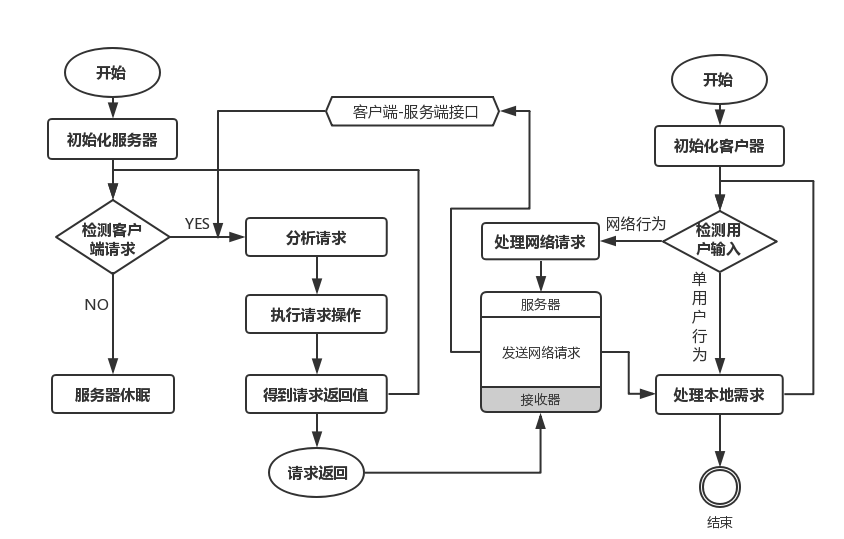
\includegraphics[width=15cm]{images/do_1}
\caption{总体流程图}
\end{figure}

我们的软件需要服务器端与客户端的交互作用,
可以从此图中看到,服务器需要保持长时间的高响应状态,
并且,从客户端输入的请求时不定时、无规律的,
所以我们的服务端在响应请求时,需要动态的根据一定时间段内的
请求数量以及请求类型进行相应的服务调整,
比如,调整自动选择的音质、画质的输出,
自动调整非紧急的下载任务,或调低相应响应速度。

需要注意的是,为了客户端的服务模型的一致性与可重用性,
网络行为与单用户行为(本地行为)有一定的重叠,
这种服务模型可以提高我们的软件行为一致性。

\newpage
\subsection{系统基本流程}
\begin{figure}[h!]
\centering
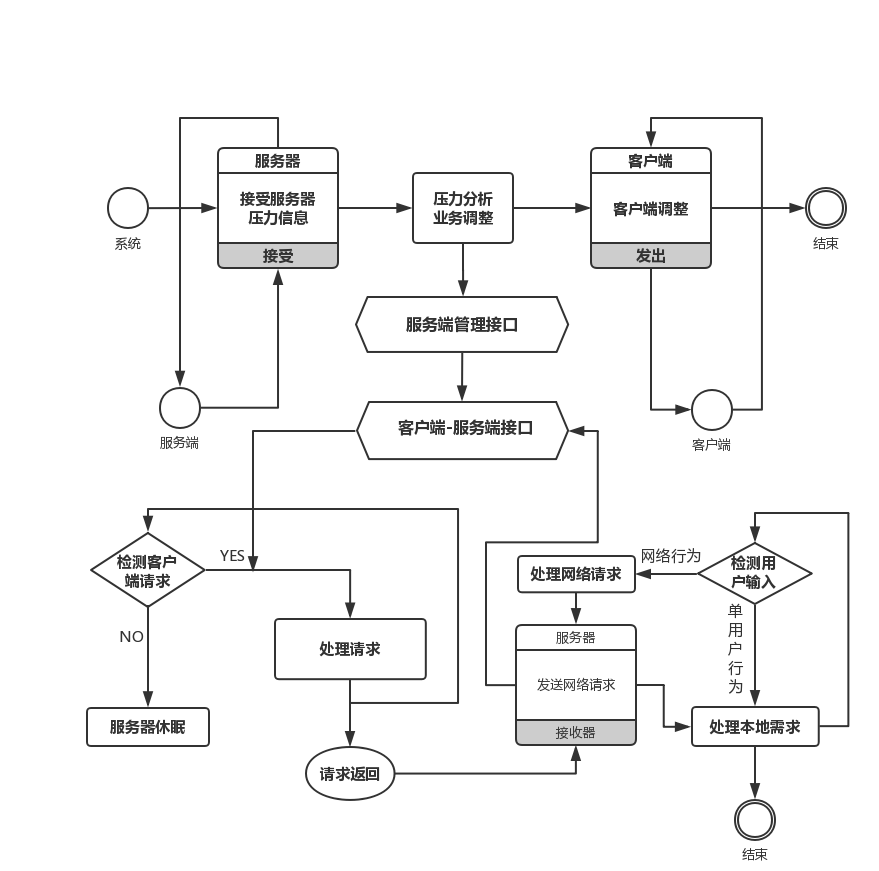
\includegraphics[width=15cm]{images/do_2}
\caption{系统基本流程图}
\end{figure}

我们的系统作为服务短语客户端之间的管理系统,
会动态的根据服务器的状态,
 当前的请求压力,对于服务端以及客户端的行为做出调整。

 如图所示,服务端和客服端对于系统同时有数据输入与输出,
 而我们的系统,根据这些信息会做出决断。

\newpage
\subsection{客户端基本流程}
\begin{figure}[h!]
\centering
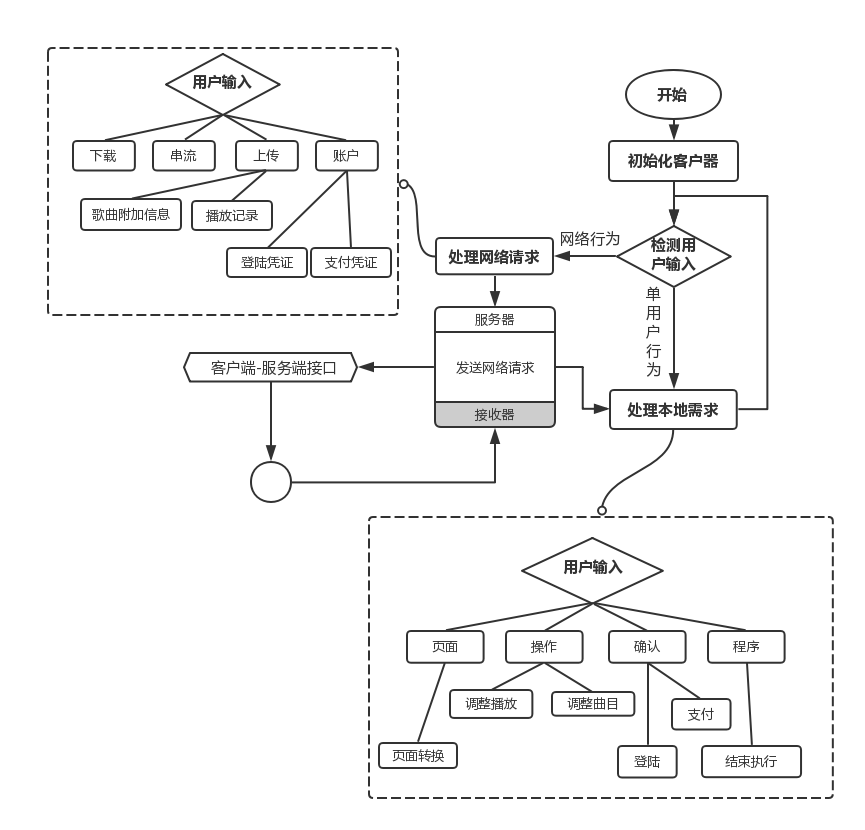
\includegraphics[width=15cm]{images/do_3}
\caption{客户端基本流程图}
\end{figure}

本图中,我们列出了客户端的基本处理流程。

可以看到,在客户端的服务流程模式中,我们需要对于网络请求,
可能有下载或串流的\textbf{大文件低频率型}请求,
也有上传用户对歌曲做出的评分、评价等
\textbf{小文件高频率型}数据需求。
对于这些不同的数据特征,需要有与服务器交互时的不同策略。

对于单用户本地输入,我们的实现方式可以较为随意,
因为满足要求即可,而不会牵扯到服务端以及系统级别的服务
的改变。

\newpage
\subsection{服务器端基本流程}
\begin{figure}[h!]
\centering
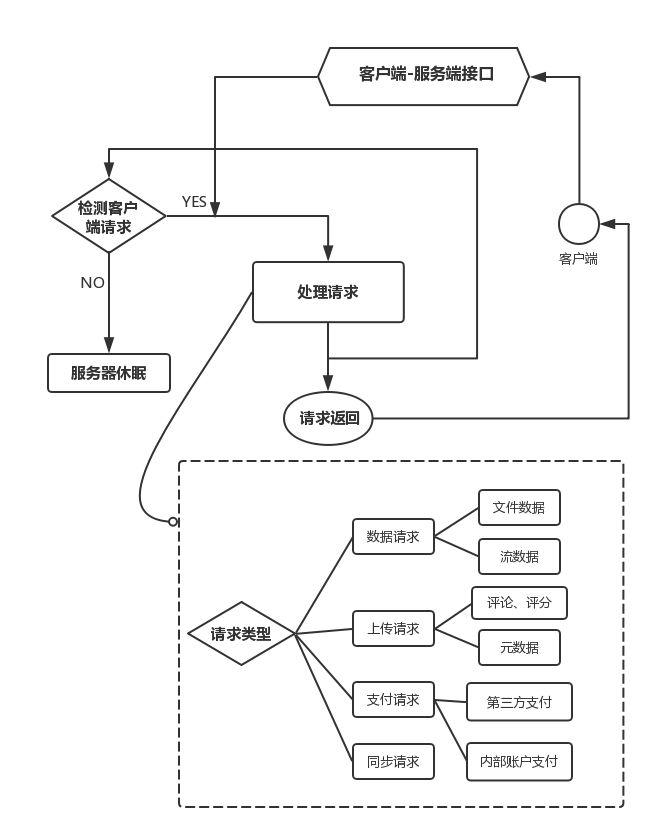
\includegraphics[width=13cm]{images/do_4}
\caption{服务端基本流程图}
\end{figure}

本图中,我们列出了服务器端的基本处理流程。

对于服务器的任务,我们可以将其大致分为四个部分,
分别对应着四种请求,即:数据请求、上传请求、
支付请求、同步请求。对于这四种请求,我们将使用不同的模块
来分别对其进行响应。

\newpage
\subsection{客户端功能具体流程}
\subsubsection{页面转换} % (fold)
\label{ssub:页面转换}
用户通过用户图形界面中的控制元素,
如,对于PC端,使用鼠标点击页面的转换按钮,
或对于移动客户端,触摸相应的按钮或大幅度两侧滑动界面,
需要使得客户端响应这样的输入,
做到相应的页面转换,
由于音乐客户端的特殊性,
我们需要满足在各个页面下够可以播放房钱正在收听的音乐,
所以,无论是网页客户端还是移动客户端,
我们都需要增加迷你播放器,
来在不是歌曲播放界面的页面中给予用户方便地控制、切换、调整播放行为的方式。
% subsubsection 页面转换 (end)

\subsubsection{歌曲操作} % (fold)
\label{ssub:歌曲操作}
歌曲操作对应于两种情形:

首先,在真实的完整播放界面中,我们需要给予用户完整的播放控制能力,
包括:
\begin{enumerate}
    \item 精确控制进度条:(在移动端)控制条的拖动速度可以通过
    触摸位置与进度条的相对垂直距离来控制,具体要求见第七章;
    \item 切换播放/暂停状态;
    \item 切换歌曲列表的播放模式:包括顺序播放、随机播放、列表循环。
    \item 下一曲/上一曲;
\end{enumerate}

而对于其他页面下的迷你播放器,功能上可以有所放松,
比如,精确控制进度条的功能可以不实现。
% subsubsection 歌曲操作 (end)

\subsubsection{登陆操作} % (fold)
\label{ssub:登陆操作}
用户在用户登录界面输入账号和密码,客户端前端需要将登录信息做严格加密后,由后端接口
向服务器端传递登录信息,并获取服务器的返回结果。
根据返回结果,需要做以下处理:
\begin{enumerate}
    \item \textbf{登录成功}:显示正确的提示信息,并对账户界面做相应的调整。
    \item \textbf{因凭据错误登陆失败}:告知用户错误的原因,并提示重试或修改密码。
    \item \textbf{因用户不存在而登录失败}:告知用户用户名不存在,并提示是否要注册账户。
    \item \textbf{服务器响应错误}:告知用户相应的信息,并提示用户检查网络状态并重试。
\end{enumerate}
% subsubsection 登陆操作 (end)

\subsubsection{支付操作} % (fold)
\label{ssub:支付操作}
对于前端完成的订单信息,客户端应该对齐进行初步验证完整性、正确性后,
进行加密并通过后端接口向服务器进行验证。
根据返回结果,可能需要做以下处理:
\begin{enumerate}
    \item \textbf{支付成功}:显示正确的提示信息,
        并对账户界面和可用歌曲的内容做相应的调整。
    \item \textbf{因账户余额不足错导致支付失败}:告知用户错误的原因,
        并提示重试或充值。
    \item \textbf{因第三方支付验证失败错导致支付失败}:告知用户错误的原因,
        并提示重试或改变支付方式。
    \item \textbf{服务器响应错误}:告知用户相应的信息,并提示用户检查网络状态并重试。
\end{enumerate}
% subsubsection 支付操作 (end)

\subsubsection{程序控制操作} % (fold)
\label{ssub:程序控制操作}
对于程序本身的控制,我们需要完成对程序的关闭、重启、更新等操作,
这些操作涉及到不同的平台的不同操作模式。而对于Web网页客户端,
往往没有这些需求,但是,由于关闭或者刷新网页产生的类似
关闭、重启的操作,也需要进行用户行为数据的记录。
% subsubsection 程序控制操作 (end)

\subsection{服务器端功能具体流程}
\subsubsection{数据请求} % (fold)
\label{ssub:数据请求}
对于客户端传递的数据请求,可以分为
文件数据和流数据两种情形:

对于文件数据,使用的技术较为传统,只需要与客户端建立稳定的HTTP/HTTPS连接,
并传递相应的文件。因为音乐文件的大小一般不会过大,所以我们一般不需要在
客户端对于单个客户端的文件数据请求建立多信道或者多线程的连接,
但是在客户端,需要对不同文件的接收做出相应的多线程支持,
但同时下载的文件个数须有一定限制,为了减少服务器压力并充分利用客户端的网络资源。

对于流数据,我们需要考虑到数据传输通道的随时可能关闭以及随时可能需要改编数据抽取位置,
所以应当对于其灵活性作出充分设计。
% subsubsection 数据请求 (end)

\subsubsection{上传请求} % (fold)
\label{ssub:上传请求}
用户在使用软件的过程中,会高频率产生上传的信息,对于评论、评分这些对应到歌曲的
信息,需要实时的对全体网络的用户产生影响,
所以我们应该建立与数据库的专用接口,并且,通过短时间内对于同一首歌的评论、评分
进行缓存、预处理,来减少对于数据库的高频访问。

而对于,用户的浏览记录、播放记录、偏好设置等等,由于没有实施改变的需求,
我们可以利用同步机制,在程序关闭、用户登出、定时器触发计时的情形下
对其进行同步,从而减少服务器压力。
% subsubsection 上传请求 (end)

\subsubsection{支付请求} % (fold)
\label{ssub:支付请求}
客户端提出的支付请求,有可能被主动篡改或者对第三方攻击者恶意篡改,
所以我们需要对其进行严格的验证。

对于账户内部支付(余额支付),我们需要验证用户的登陆凭据,以及
账户数据库内的余额信息是否足够支付订单。对于可疑的订单行为
(如高频购买、重复购买、数额巨大订单这样的客户端理应不可能
发出的订单信息)
我们应对其进行黑名单阻挡。

对于第三方支付的账单,我们需要通过第三方支付平台的相应接口来
对其进行正确性、完整性的审查,并做出正确的反馈。
% subsubsection 支付请求 (end)

\newpage
\section{功能结构设计}
\subsection{整体结构}

我们的系统分为以下模块:

\begin{figure}[h!]
\centering
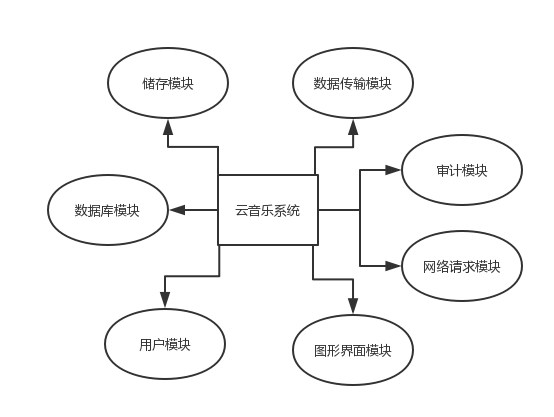
\includegraphics[width=13cm]{images/do_5}
\caption{系统模块结构图}
\end{figure}

\begin{table}[h]
\centering
\caption{系统模块结构表} 
\begin{tabular}{|c|c|}
    \hline
    模块ID & 模块名称 \\
    \hline
    M.CLOUDMUSIC.001 & 储存模块 \\
    M.CLOUDMUSIC.002 & 数据库模块 \\
    M.CLOUDMUSIC.003 & 用户模块 \\
    M.CLOUDMUSIC.004 & 图形界面模块 \\
    M.CLOUDMUSIC.005 & 数据传输模块 \\
    M.CLOUDMUSIC.006 & 审计模块 \\
    M.CLOUDMUSIC.007 & 网络请求模块 \\
    \hline
\end{tabular}
\end{table}

如图和表所示,我们分别简单描述这些模块的作用和范围:

\subsection{M.CLOUDMUSIC.001 储存模块}
\begin{itemize}
    \item 储存歌曲文件;
    \item 储存歌曲元信息,如评论、评分、下载数据、支付数据;
    \item 存储网络缓存;
    \item 存储数据库文件本身。
\end{itemize}

\subsection{M.CLOUDMUSIC.002 数据库模块}
\begin{itemize}
    \item 根据用户的请求,生成不同的数据库查询语句;
    \item 检测用户权限是否满足,若满足则发送给数据库并接收结果,否则报告错误
        并向审计模块报告越权行为;
    \item 对数据库进行高频率的更新,需要对特定用途的查询或更新设计专用的
        存储过程或触发器;
    \item 定时审计,需要与审计模块密切联系。
\end{itemize}

\subsection{M.CLOUDMUSIC.003 用户模块}
\begin{itemize}
    \item 存储用户的信息;
    \item 响应高频度的用户登录凭证验证查询任务;
    \item 动态更新用户信息的变化;
    \item 对于新用户注册,要及时进行数据更新,保证可用性。
\end{itemize}

\subsection{M.CLOUDMUSIC.004 图形界面模块}
\begin{itemize}
    \item 处理用户与图形界面的交互;
    \item 处理前端所执行的结果向服务端的发送;
    \item 处理后端接收到的服务器命令对于界面的实时变化;
    \item 对于较复杂的界面交互、动画,需要平衡性能与效果。
\end{itemize}

\subsection{M.CLOUDMUSIC.005 数据传输模块}
\begin{itemize}
    \item 对于高频小文件(HFLS, High Frequency Low Size)
        传输,保证高可用、低延迟;
    \item 对于低频大文件(LFHS, Low Frequency High Size)
        传输,保证高带宽、低重传;
\end{itemize}

\subsection{M.CLOUDMUSIC.006 审计模块}
\begin{itemize}
    \item 审计数据库模块的越权查询行为;
    \item 审计支付过程中的可以订单、可疑账户;
    \item 审计网络请求模块中的受篡改请求、恶意请求(如
        分布式拒绝服务(DDoS:Distributed Denial of Service))。
\end{itemize}

\subsection{M.CLOUDMUSIC.007 网络请求模块}
\begin{itemize}
    \item 处理服务器与客户端之间的请求交互;
    \item 处理分布式储存系统之间的同步、传输请求;
    \item 处理本地ISP与顶级ISP之间的网络服务调配。
\end{itemize}

\newpage

\section{功能需求与程序代码的关系}
\begin{table}[htbp]
\centering
\caption{功能需求与程序代码的关系表} \label{tab:requirement-module}


\begin{tabular}{|c|c|c|c|c|c|c|c|}
    \hline
    功能 &              储存 & 数据库 & 用户 & 图形界面 & 数据传输 & 审计 & 网络请求 \\
    \hline
    SYS.001 客户端启动 &   Y &    •   & •    &     Y    &    •     &  •   &   •      \\
    \hline
    SYS.002 客户端关闭 &   Y &    •   & •    &     Y    &    •     &  •   &   •      \\
    \hline
    SYS.003 客户端升级 &   Y &    •   & •    &     Y    &    Y     &  •   &   Y      \\
    \hline
    USER.001 用户登录  &   Y &    Y   & Y    &     Y    &    •     &  Y   &   Y      \\
    \hline
    USER.002 用户注册  &   Y &    Y   & Y    &     Y    &    •     &  Y   &   Y      \\
    \hline
    USER.003 用户注销  &   Y &    Y   & Y    &     Y    &    •     &  Y   &   Y      \\
    \hline
APP.001 生成主页界面   &   • &    •   & •    &     Y    &    •     &  •   &   •      \\
    \hline
APP.002 生成音乐集界面 &   • &    •   & •    &     Y    &    •     &  •   &   •      \\
    \hline
APP.003 生成音乐播放界面 & • &    •   & •    &     Y    &    •     &  •   &   •      \\
    \hline
APP.004 生成音乐推荐界面 & • &    Y   & Y    &     Y    &    Y     &  •   &   Y      \\
    \hline
APP.005 生成账户界面   &   • &    Y   & Y    &     Y    &    Y     &  •   &   Y      \\
    \hline
APP.006 生成设置界面   &   • &    •   & •    &     Y    &    •     &  •   &   •      \\
    \hline
MUSIC.001 音乐播放控制 &   Y &    Y   & •    &     Y    &    Y     &  •   &   Y      \\
    \hline
MUSIC.002 音乐串流控制 &   Y &    Y   & •    &     Y    &    Y     &  •   &   Y      \\
    \hline
MUSIC.003 音乐下载控制 &   Y &    Y   & •    &     Y    &    Y     &  •   &   Y      \\
    \hline
    SHOP.001 购买音乐  &   • &    Y   & Y    &     Y    &    •     &  Y   &   Y      \\
    \hline
    SHOP.002 购买订阅  &   • &    Y   & Y    &     Y    &    •     &  Y   &   Y      \\
    \hline
SYNC.001 数据同步上传  &   Y &    •   & Y    &     •    &    •     &  Y   &   Y      \\
    \hline
SYNC.002 数据同步下载  &   Y &    •   & Y    &     •    &    •     &  Y   &   Y      \\
    \hline

\end{tabular}
\note{各项功能需求的实现与各个程序模块的分配关系}
\end{table}
\chapter{接口设计}
\section{外部接口}
比如说需要用到支付宝等外部支付系统,接口应当如何封装。

\subsection{支付宝接口}
详细讲述不同的接口(查询状态、支付交易、获取回执等)

\section{内部接口}
内部模块/系统之间的交互的接口。
\chapter{数据结构设计}
\section{逻辑结构设计}
\subsection{用户数据结构}

class User:             用户类\\
\indent \indent    UID : int           每个账户的唯一标识符\\
\indent \indent    Username: String    账户用户名\\
\indent \indent    Password: String    账户密码\\
\indent \indent    AccessToken: String 每次登陆生成的 Token

\subsection{歌曲数据结构}

class Song:\\
\indent \indent   SID : int           每首歌曲的唯一标识符\\
\indent \indent   Name : String       歌曲名\\
\indent \indent   Author : String list 歌曲的作者名\\
\indent \indent   AID : int           歌曲的专辑标识符\\
\indent \indent   Available : bool    歌曲是否已下架\\
\indent \indent   Score : float       歌曲评分\\
\\
class Album:\\
\indent \indent    AID : int           专辑的标识符\\
\indent \indent    Name : String       专辑的名称\\
\indent \indent    Songs : int list list   顺序排列的歌曲曲目,用标识符表示\\
\indent \indent                            (每一列表示一张碟)
\indent \indent    Release : Datetime  专辑公开日期

\subsection{购买情况数据结构}

class PurchaseSong:\\
\indent \indent    SID : int           歌曲的标识符\\
\indent \indent    UID : int           用户的标识符\\
\indent \indent    ListenAvailable : bool    用户是否能够听该曲\\
\indent \indent    DownloadAvailable : bool  用户能否下载该曲\\
\indent \indent    ListenUntil : Datetime    听歌的有效期限\\
\indent \indent    DownloadUntil : Datetime  下载的有效期限

\subsection{评论数据结构}

class Comment:\\
\indent \indent    SID : int           评论所在歌曲的标识符\\
\indent \indent    UID : int           评论者的标识符\\
\indent \indent    Text : String       评论的内容\\
\indent \indent    Date : Datetime     评论的时间

\subsection{本地缓存数据结构}

class CacheState:       本地的缓存状况\\
\indent \indent    type : enum{Music, AlbumImage, UserImage}
\indent \indent                        缓存内容的种类\\
\indent \indent    ID : int            资源的标识符\\
\indent \indent    Ready : bool        资源是否已下载到本地\\
\indent \indent    Size : int          缓存资源的大小\\
\indent \indent    Downloaded : int    已下载部分的大小

\section{物理结构设计}
各数据结构无特殊物理结构要求。

\section{数据结构与程序模块的关系}
\begin{table}[htbp]
\centering
\caption{客户端数据结构与程序代码的关系表} \label{tab:datastructure-module-client}
\begin{tabular}{|c|c|c|c|c|c|}
    \hline
    模块$\backslash$ 数据结构 & 用户 & 评论 & 歌曲 & 购买情况 & 本地缓存 \\
    \hline
    储存 & Y & Y & Y & Y & Y \\
    \hline
    数据库 & Y & Y & Y & Y & . \\
    \hline
    用户 & Y & . & . & . & . \\
    \hline
    图形界面 & Y & Y & Y & Y & Y \\
    \hline
    数据传输 & . & . & . & . & Y \\
    \hline
    审计 & . & . & . & . & . \\
    \hline
    网络请求 & Y & Y & Y & Y & Y \\
    \hline
\end{tabular}
\note{客户端各项数据结构的实现与各个程序模块的分配关系}
\end{table}

\begin{table}[htbp]
    \centering
    \caption{服务端数据结构与程序代码的关系表} \label{tab:datastructure-module-server}
    \begin{tabular}{|c|c|c|c|c|c|}
        \hline
        模块$\backslash$ 数据结构 & 用户 & 评论 & 歌曲 & 购买情况 & 本地缓存 \\
        \hline
        储存 & Y & Y & Y & Y & . \\
        \hline
        数据库 & Y & Y & Y & Y & . \\
        \hline
        用户 & Y & . & . & . & . \\
        \hline
        图形界面 & . & . & . & . & . \\
        \hline
        数据传输 & . & . & . & . & . \\
        \hline
        审计 & Y & . & . & Y & . \\
        \hline
        网络请求 & Y & Y & Y & Y & . \\
        \hline
    \end{tabular}
    \note{服务器端各项数据结构的实现与各个程序模块的分配关系}
    \end{table}
\chapter{数据库设计}
\section{数据库环境说明}
本系统的数据系统采用PostgreSQL数据库系统。


\section{数据库的命名规则}
\begin{itemize}
	\item 不允许使用缩写
	\item 表名使用单数形式。对于有关联的表,属性名用表名+id的方式来标明这是外表的一个主键
	\item 字段名字不带前缀
\end{itemize}

\section{逻辑设计}

数据模型满足3NF\\
\newpage

\begin{figure}[ht]
	\centering
	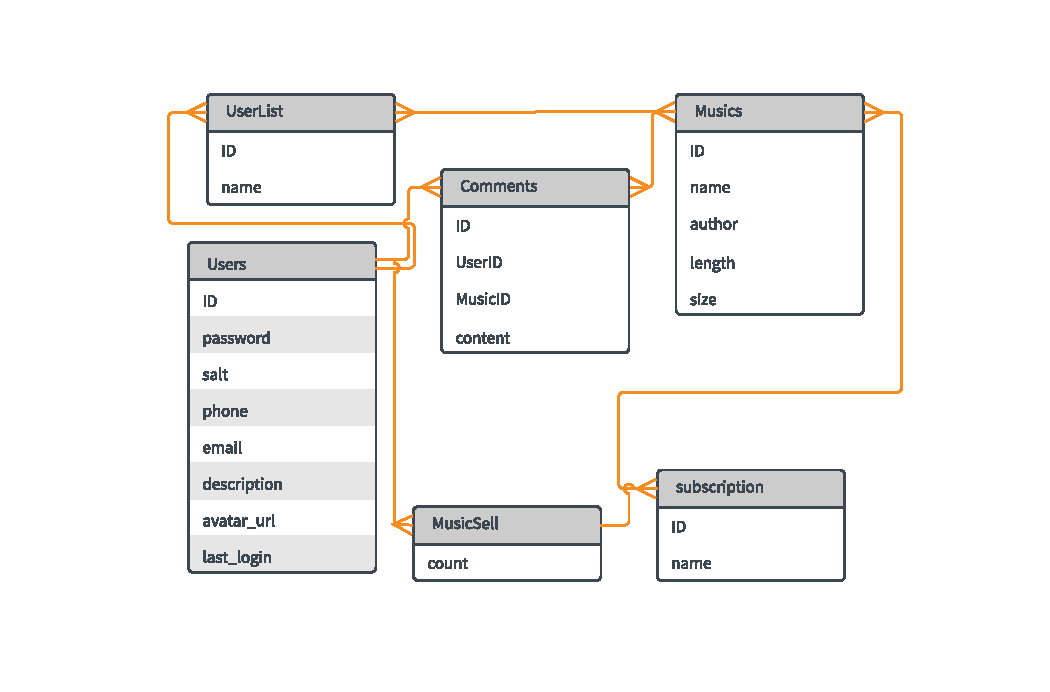
\includegraphics[width=14cm]{database_ER}
	\caption{ER模型图}\label{fig:ER}
\end{figure}

\section{物理设计}

\subsection{数据库产品}

数据库采用了PostgreSQL,由于暂时数据访问量不大,所以不使用分布式结构。

\subsection{实体属性、类型、精度}

\subsubsection{用户数据表设计}

用户数据表保存了用户的基本信息

\begin{table}[htbp]
\centering
\caption{用户数据表Users设计} \label{tab:users-database}
\begin{tabular}{|c|c|c|c|c|}
    \hline
    字段名 & 类型 & 大小 & 说明 & 备注 \\
    \hline
    ID & char & 64 & 用户的唯一标识符 & 主键\\
    \hline
    password & char & 256 & 用户密码的哈希 & · \\
    \hline
    salt & char & 256 & 盐 & · \\
    \hline
    phone & char & 18 & 电话号码 & 外键 \\
    \hline
    email & char & 32 & 电子邮箱 & · \\
    \hline
    description & char & 1024 & 个人自述 & · \\
    \hline
    avatar\_url & char & 256 & 头像地址 & · \\
    \hline
    last\_login & timestamp & 32 & 上次登录时间 & · \\
    \hline
    music\_lists & json & var & 自定义歌单的集合 & . \\
    \hline
\end{tabular}
\note{用户数据表Users设计}
\end{table}

\subsubsection{电话用户对应关系表PhoneToUser设计}

电话用户对应关系表保存了用户电话到用户ID的对应关系

\begin{table}[htbp]
\centering
\caption{电话用户对应关系表PhoneToUser设计} \label{tab:phone-user-database}
\begin{tabular}{|c|c|c|c|c|}
    \hline
    字段名 & 类型 & 大小 & 说明 & 备注 \\
    \hline
    phone & char & 18 & 用户电话号码 & 主键\\
    \hline
    user\_id & char & 64 & 对应用户 & 外键,来自表Users \\
    \hline
\end{tabular}
\note{电话用户对应关系表PhoneToUser设计}
\end{table}

\subsubsection{音乐信息数据库Musics设计}

音乐信息数据库保存了音乐的信息

\begin{table}[htbp]
	\centering
	\caption{音乐信息数据库Musics设计} \label{tab:music-database}
	\begin{tabular}{|c|c|c|c|c|}
		\hline
		字段名 & 类型 & 大小 & 说明 & 备注 \\
		\hline
		ID & char & 64 & 音乐唯一标识符 & 主键\\
		\hline
		name & char & 64 & 音乐名称 & · \\
		\hline
		author & char & 64 & 作者 & · \\
		\hline
		length & smallint & 16 & 时长(秒) & · \\
		\hline
		size & int & 32 & 大小(字节) & · \\
		\hline
	\end{tabular}
	\note{音乐信息数据库Musics设计}
\end{table}

\subsubsection{订阅信息数据库Subscriptions设计}

订阅信息数据库保存了订阅的信息

\begin{table}[htbp]
	\centering
	\caption{订阅信息数据库Subscriptions设计} \label{tab:subscription-database}
	\begin{tabular}{|c|c|c|c|c|}
		\hline
		字段名 & 类型 & 大小 & 说明 & 备注 \\
		\hline
		ID & char & 64 & 订阅唯一标识符 & 主键\\
		\hline
		name & char & 64 & 订阅名称 & · \\
		\hline
		contents & json & var & 包含的音乐的集合  & · \\
		\hline
	\end{tabular}
	\note{订阅信息数据库Subscriptions设计}
\end{table}

\subsubsection{用户音乐购买信息MusicSells设计}

用户音乐购买信息保存了相当于订阅信息倒排索引的信息

\begin{table}[htbp]
	\centering
	\caption{用户音乐购买信息MusicSells设计} \label{tab:music-sell-database}
	\begin{tabular}{|c|c|c|c|c|}
		\hline
		字段名 & 类型 & 大小 & 说明 & 备注 \\
		\hline
		user\_ID & char & 64 & 用户ID & 主键\\
		\hline
		music\_ID & char & 64 & 音乐ID & 主键 \\
		\hline
		count & smallint & 8 & 累计次数  & · \\
		\hline
	\end{tabular}
	\note{用户音乐购买信息MusicSells设计}
\end{table}

\subsubsection{自定义歌单数据库MusicList设计}

自定义歌单数据库保存了歌单的信息

\begin{table}[htbp]
	\centering
	\caption{自定义歌单数据库MusicList设计} \label{tab:music-list-database}
	\begin{tabular}{|c|c|c|c|c|}
		\hline
		字段名 & 类型 & 大小 & 说明 & 备注 \\
		\hline
		ID & char & 64 & 歌单唯一标识符 & 主键\\
		\hline
		name & char & 64 & 歌单名称 & · \\
		\hline
		contents & json & var & 包含的音乐的集合  & · \\
		\hline
	\end{tabular}
	\note{自定义歌单数据库MusicList设计}
\end{table}

\subsubsection{用户评论Comments设计}

自定义歌单数据库保存了歌单的信息

\begin{table}[htbp]
	\centering
	\caption{用户评论Comments设计} \label{tab:music-list-database}
	\begin{tabular}{|c|c|c|c|c|}
		\hline
		字段名 & 类型 & 大小 & 说明 & 备注 \\
		\hline
		ID & char & 64 & 用户评论唯一标识符 & 主键 \\
		\hline
		UserID & char & 64 & 用户ID & 外键 \\
		\hline
		MusicID & char & 64 & 歌曲ID & 外键 \\
		\hline
		comment & char & 512 & 用户对歌曲的评论  & · \\
		\hline
	\end{tabular}
	\note{用户评论Comments设计}
\end{table}

\section{安全性设计}	
通过合理设置权限,只有管理员和应用程序账号
能修改表的数据和读取用户隐私相关的数据。同时,数据库进行定时热备份,保证了数据库
即使在服务器出问题丢失数据的情况下迅速恢复。

\section{数据库管理与维护说明}
监视数据库进程,如果出现无法连接马上告警。

定时更新数据库安全补丁。
%!TEX root = ../main.tex

\chapter{界面设计}
\section{客户端界面}

\subsection{PC 客户端界面} % (fold)
\label{sub:pc_客户端界面}

本小节讲述在PC客户端上,用户界面应具有的设计需求。

\begin{enumerate}
	\item \textbf{要求的屏幕格式}:
		PC客户端支持大于$800 \times 600$ 分辨率的屏幕,并对根据屏幕大小以及系统
		设定的屏幕元素放大比例做自动适应;
	\item \textbf{使用方式}:
		对于一般的用户,我们的产品使用逻辑与一般的PC软件一致,
			用户不需要主动学习便可学会使用它,
		同时,我们也会在安装后附上使用说明书,来保证用户可以方便使用;
	\item \textbf{页面规划}: 
	\begin{itemize}
		\item 主页界面的用户界面设计,请参考图\ref{fig:desttop_home};
		\item 音乐播放界面的用户界面设计,请参考图\ref{fig:desttop_music};
		\item 音乐集查看界面的用户界面设计,请参考图\ref{fig:desttop_collection};
	\end{itemize}
\end{enumerate}

\newpage
\begin{figure}[h!]
  \centering

  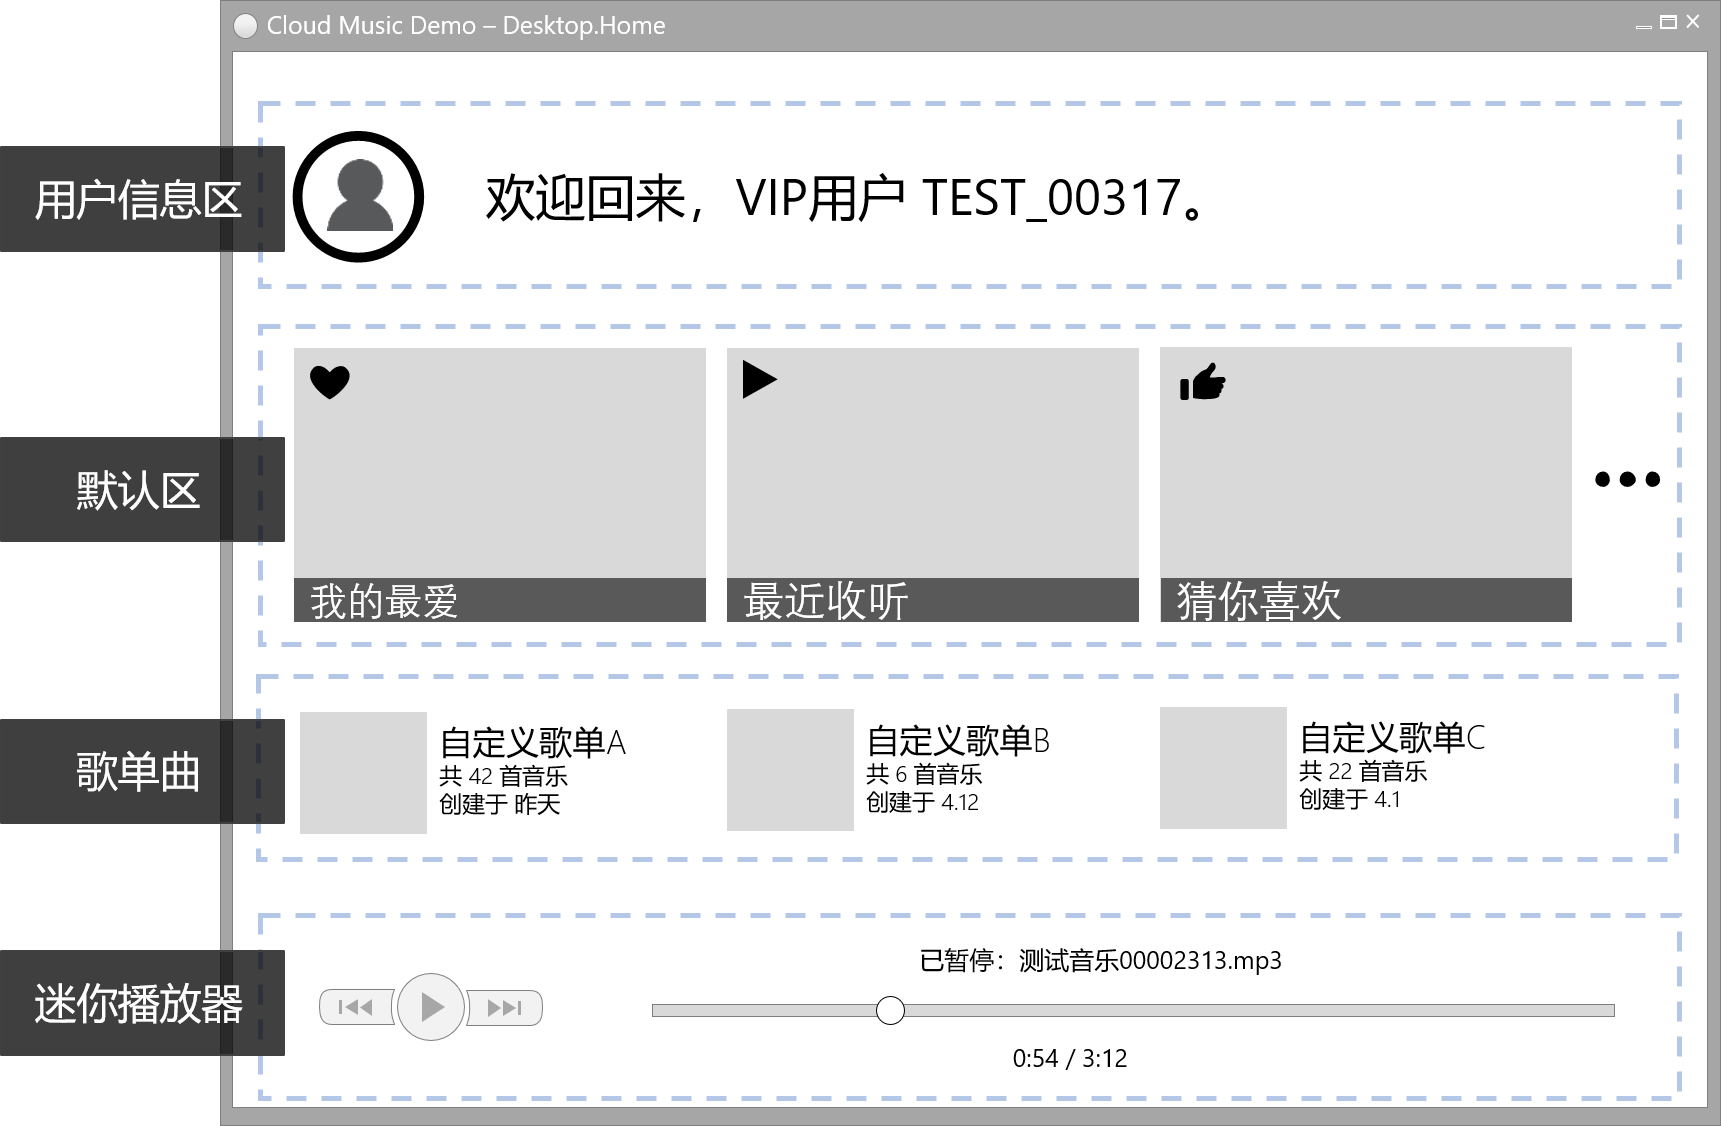
\includegraphics[width=.95\linewidth]{figures/desttop_home}

  \caption{  \label{fig:desttop_home}
  		PC客户端主页(Home Page)用户界面设计图
    }
\end{figure}

\begin{figure}[h!]
  \centering
 
  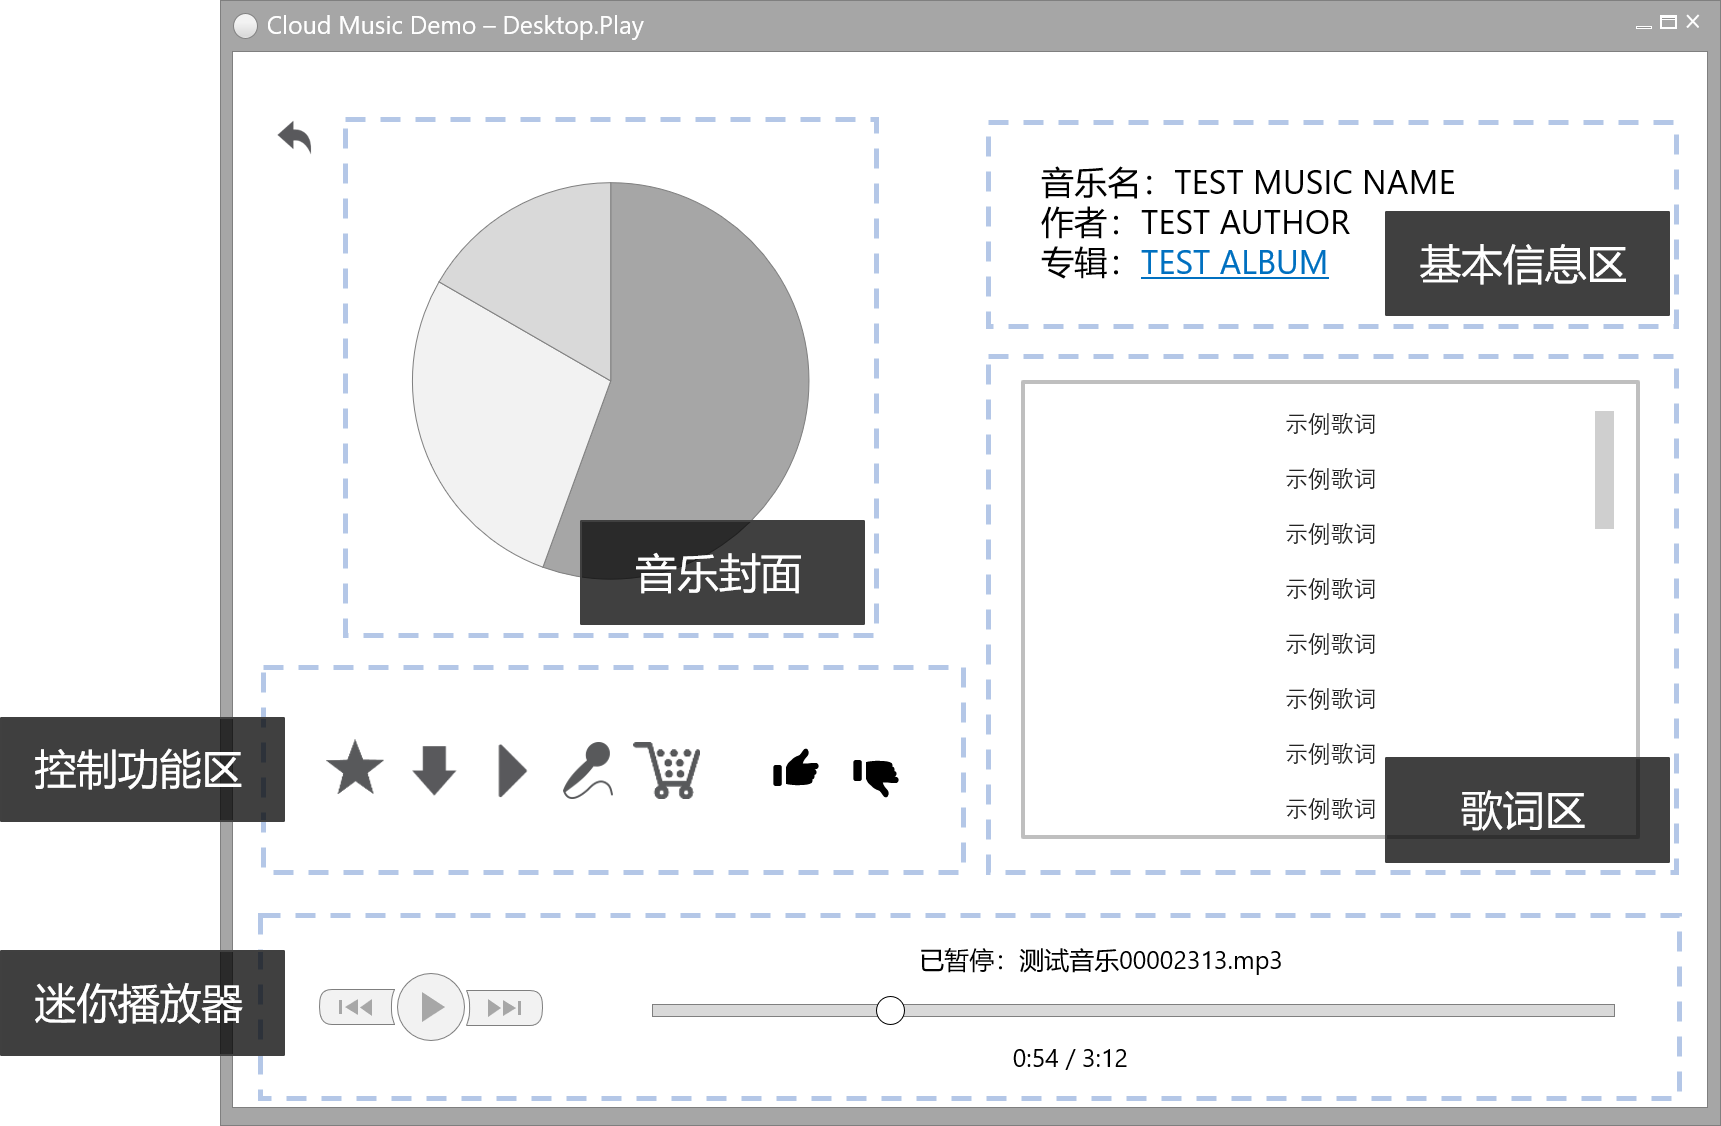
\includegraphics[width=.95\linewidth]{figures/desttop_music}

  \caption{ \label{fig:desttop_music}
  		PC客户端音乐播放界面用户界面设计图
    }
\end{figure}

\newpage
\begin{figure}[h!]
  \centering

  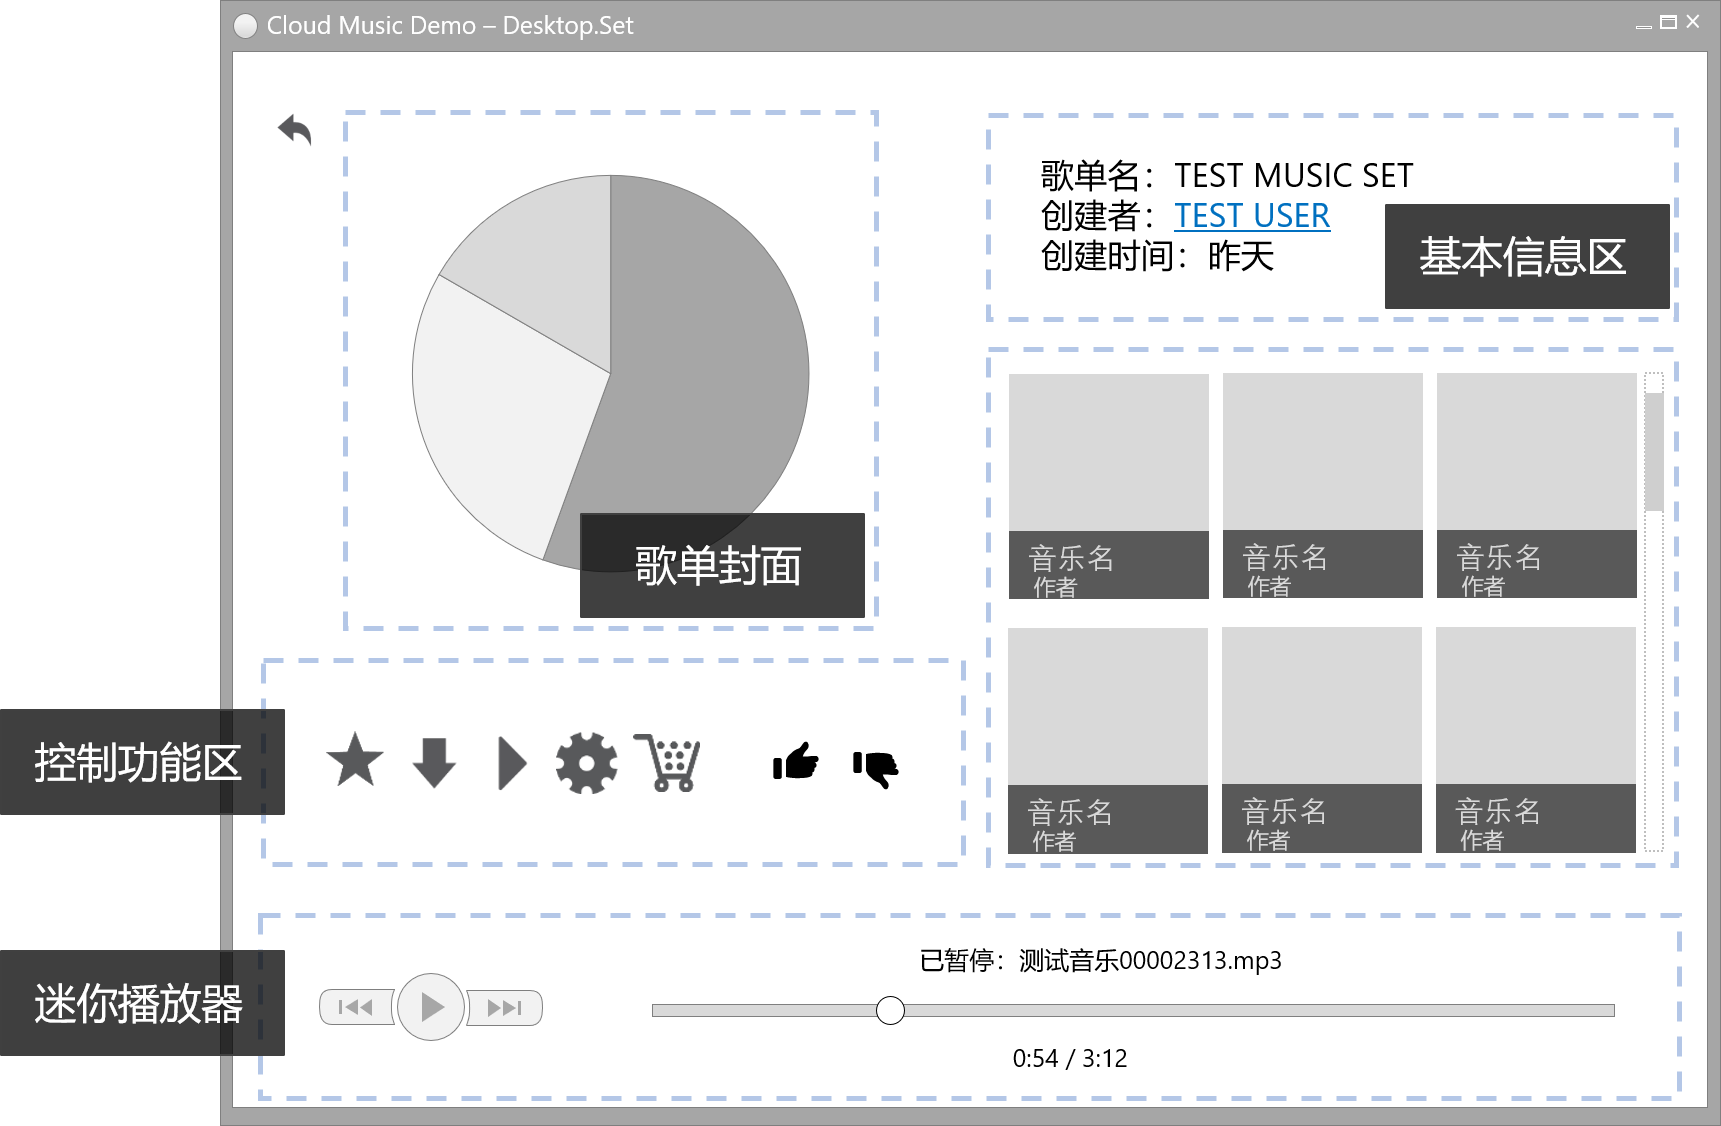
\includegraphics[width=.95\linewidth]{figures/desttop_collection}

  \caption{  \label{fig:desttop_collection}
  		PC客户端音乐集展示用户界面设计图
    }
\end{figure}

% subsection pc_客户端界面 (end)
\subsection{移动客户端界面} % (fold)
\label{sub:移动客户端界面}
\begin{enumerate}
	\item \textbf{要求的屏幕格式}:
		PC客户端支持大于$1334 \times 750$ 分辨率的移动设备屏幕,并对根据屏幕大小以及系统
		设定的屏幕元素放大比例做自动适应;
	\item \textbf{使用方式}:
		对于一般的用户,我们的产品使用逻辑与一般的移动设备软件一致,
			用户不需要主动学习便可学会使用它,
		同时,我们也会在安装后附上使用说明书,来保证用户可以方便使用;
	\item \textbf{页面规划}: 
	\begin{itemize}
		\item 主页界面的用户界面设计,请参考图\ref{fig:mobile_home};
		\item 音乐播放界面的用户界面设计,请参考图\ref{fig:mobile_music};
		\item 音乐集查看界面的用户界面设计,请参考图\ref{fig:mobile_collection};
	\end{itemize}
\end{enumerate}

\begin{figure}[h!]
  \centering

  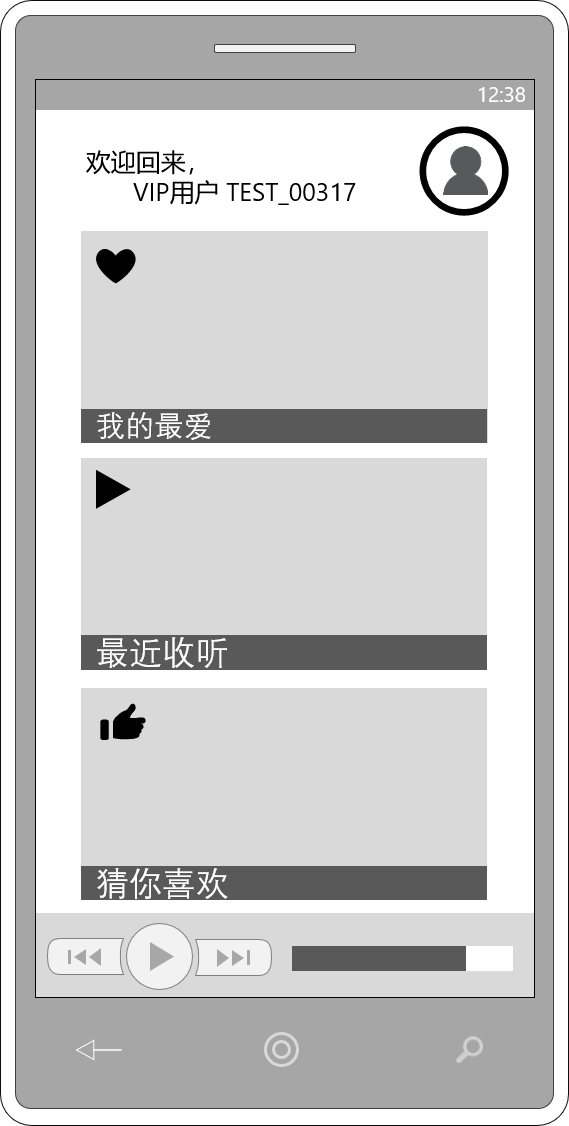
\includegraphics[width=.33\linewidth]{figures/mobile_home}

  \caption{  \label{fig:mobile_home}
  		移动客户端主页(Home Page)用户界面设计图
    }
\end{figure}

\begin{figure}[h!]
  \centering
 
  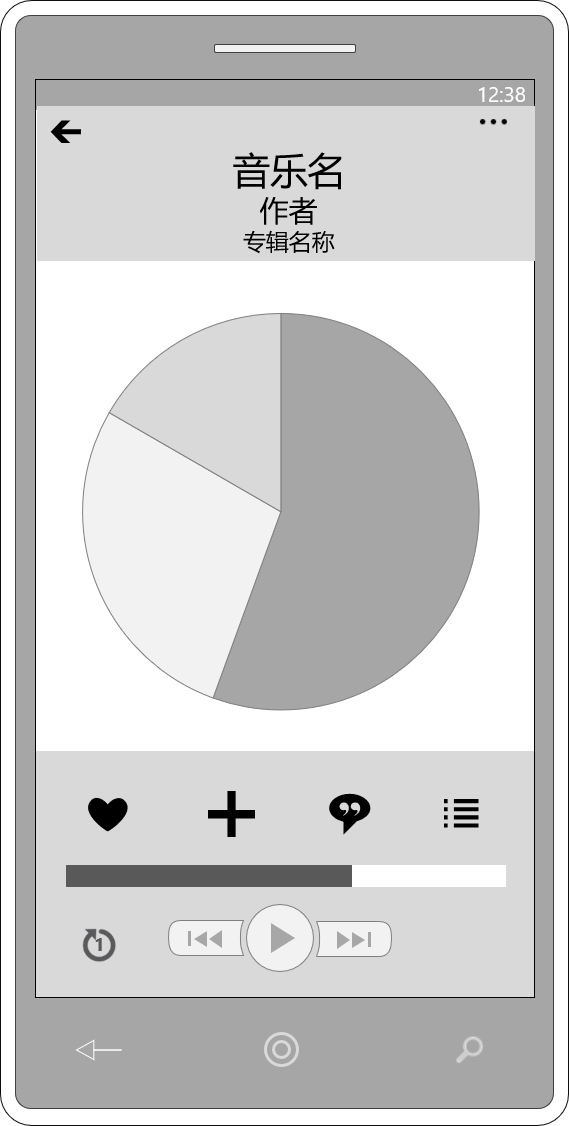
\includegraphics[width=.33\linewidth]{figures/mobile_music}

  \caption{ \label{fig:mobile_music}
  		移动客户端音乐播放界面用户界面设计图
    }
\end{figure}

\begin{figure}[h!]
  \centering

  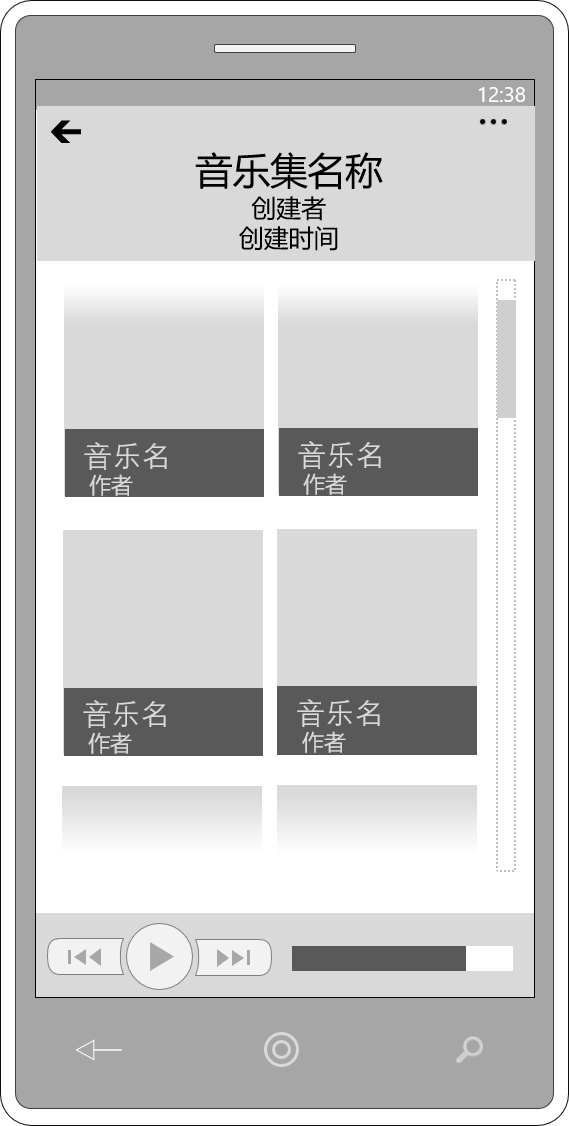
\includegraphics[width=.33\linewidth]{figures/mobile_collection}

  \caption{  \label{fig:mobile_collection}
  		移动客户端音乐集展示用户界面设计图
    }
\end{figure}
% subsection 移动客户端界面 (end)

\newpage
\R {
\subsection{私人空间界面及动态界面} % (fold)
	\begin{enumerate}
	\item \textbf{使用方式}:
		私人空间中,用户的基本信息和两种表现形式。
		首先是``他/她的歌单'',显示该用户创建的歌单,并可以进行点赞操作。
		然后是``他/她的动态'',可以展示该用户发出的动态,并可以进行评论和点赞。
		以上点赞和评论的数量会被显示。
	\item \textbf{页面规划}: 
	\begin{itemize}
		\item 私人空间-歌单界面设计,请参考图\ref{fig:mobile_user1};
		\item 私人空间-动态界面设计,请参考图\ref{fig:mobile_user2};
	\end{itemize}
\end{enumerate}
}
\newpage
\begin{figure}[h!]
  \centering
  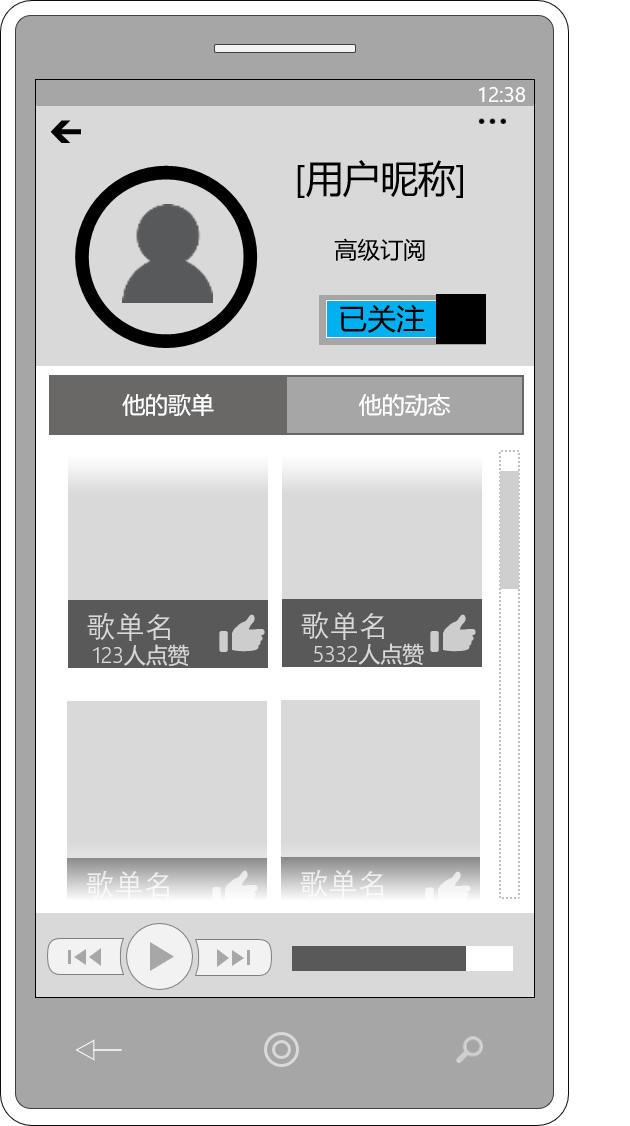
\includegraphics[width=.37\linewidth]{figures/mobile_user1}
  \caption{  \label{fig:mobile_user1}
	\R{私人空间-歌单界面设计图}
    }
\end{figure}

\begin{figure}[h!]
  \centering
  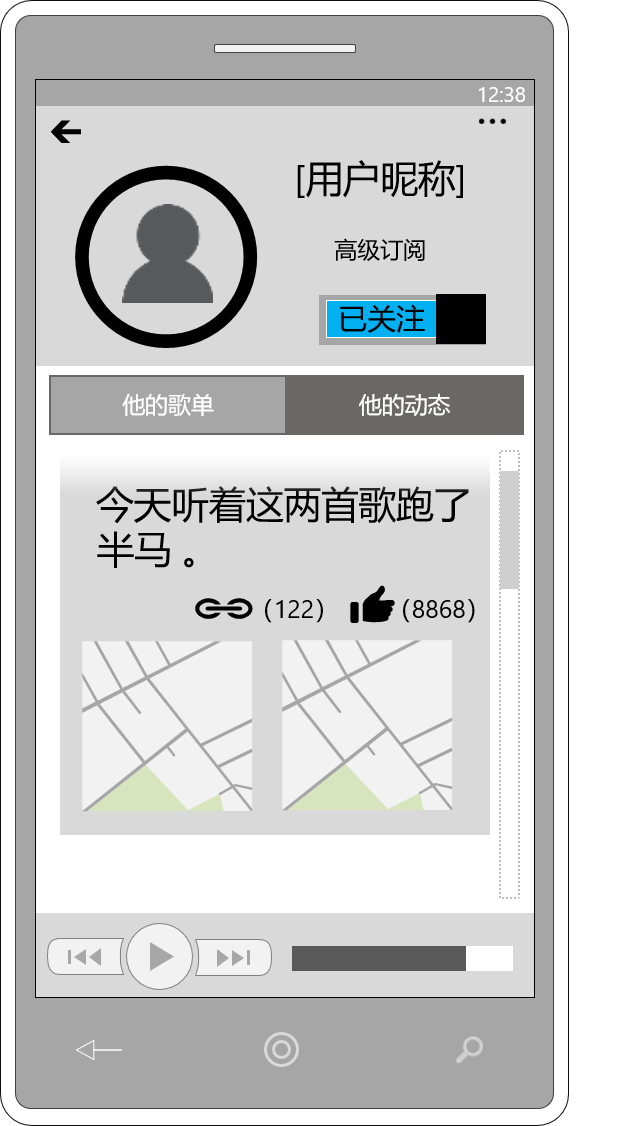
\includegraphics[width=.37\linewidth]{figures/mobile_user2}
  \caption{  \label{fig:mobile_user2}
	\R{私人空间-动态界面设计图}
    }
\end{figure}

\newpage

\R {
\subsection{K歌功能界面} % (fold)
	\begin{enumerate}
	\item \textbf{使用方式}:
		在K歌功能界面中,用户可以进行录制歌曲。
		我们将歌词放置在界面中,
		并且可以快速跳转到对应的歌词的时间轴位置。
		并且,提供了重录上一句的快捷按钮。
	\item \textbf{页面规划}: 
	\begin{itemize}
		\item K歌界面设计,请参考图\ref{fig:mobile_K};
	\end{itemize}
\end{enumerate}
}
\begin{figure}[h!]
  \centering
  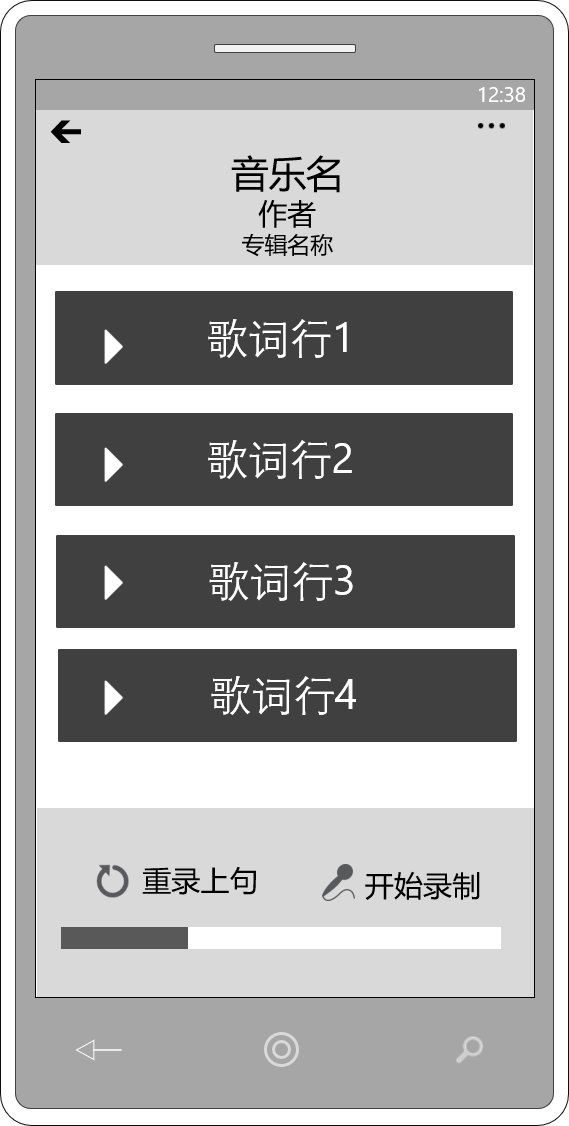
\includegraphics[width=.37\linewidth]{figures/mobile_K}
  \caption{  \label{fig:mobile_K}
	\R{K歌界面设计图}
    }
\end{figure}

\newpage

\subsection{网页客户端用户界面} % (fold)

\begin{enumerate}
	\item \textbf{要求的屏幕格式}:
		网页客户端支持大于$800 \times 600$ 分辨率的通用网页浏览器,
		并对根据屏幕大小以及浏览器设定的屏素放大比例做自动适应;
	\item \textbf{使用方式}:
		对于一般的用户,我们的产品使用逻辑与一般的网页一致,
			用户不需要主动学习便可学会使用它,
		同时,我们也会在安装后附上使用说明书,来保证用户可以方便使用;
	\item \textbf{页面规划}: 
	\begin{itemize}
		\item 主页界面的用户界面设计,请参考图\ref{fig:web_home};
		\item 音乐播放界面的用户界面设计,请参考图\ref{fig:web_music};
		\item 音乐集查看界面的用户界面设计,请参考图\ref{fig:web_collection};
	\end{itemize}
\end{enumerate}

\begin{figure}[h!]
  \centering

  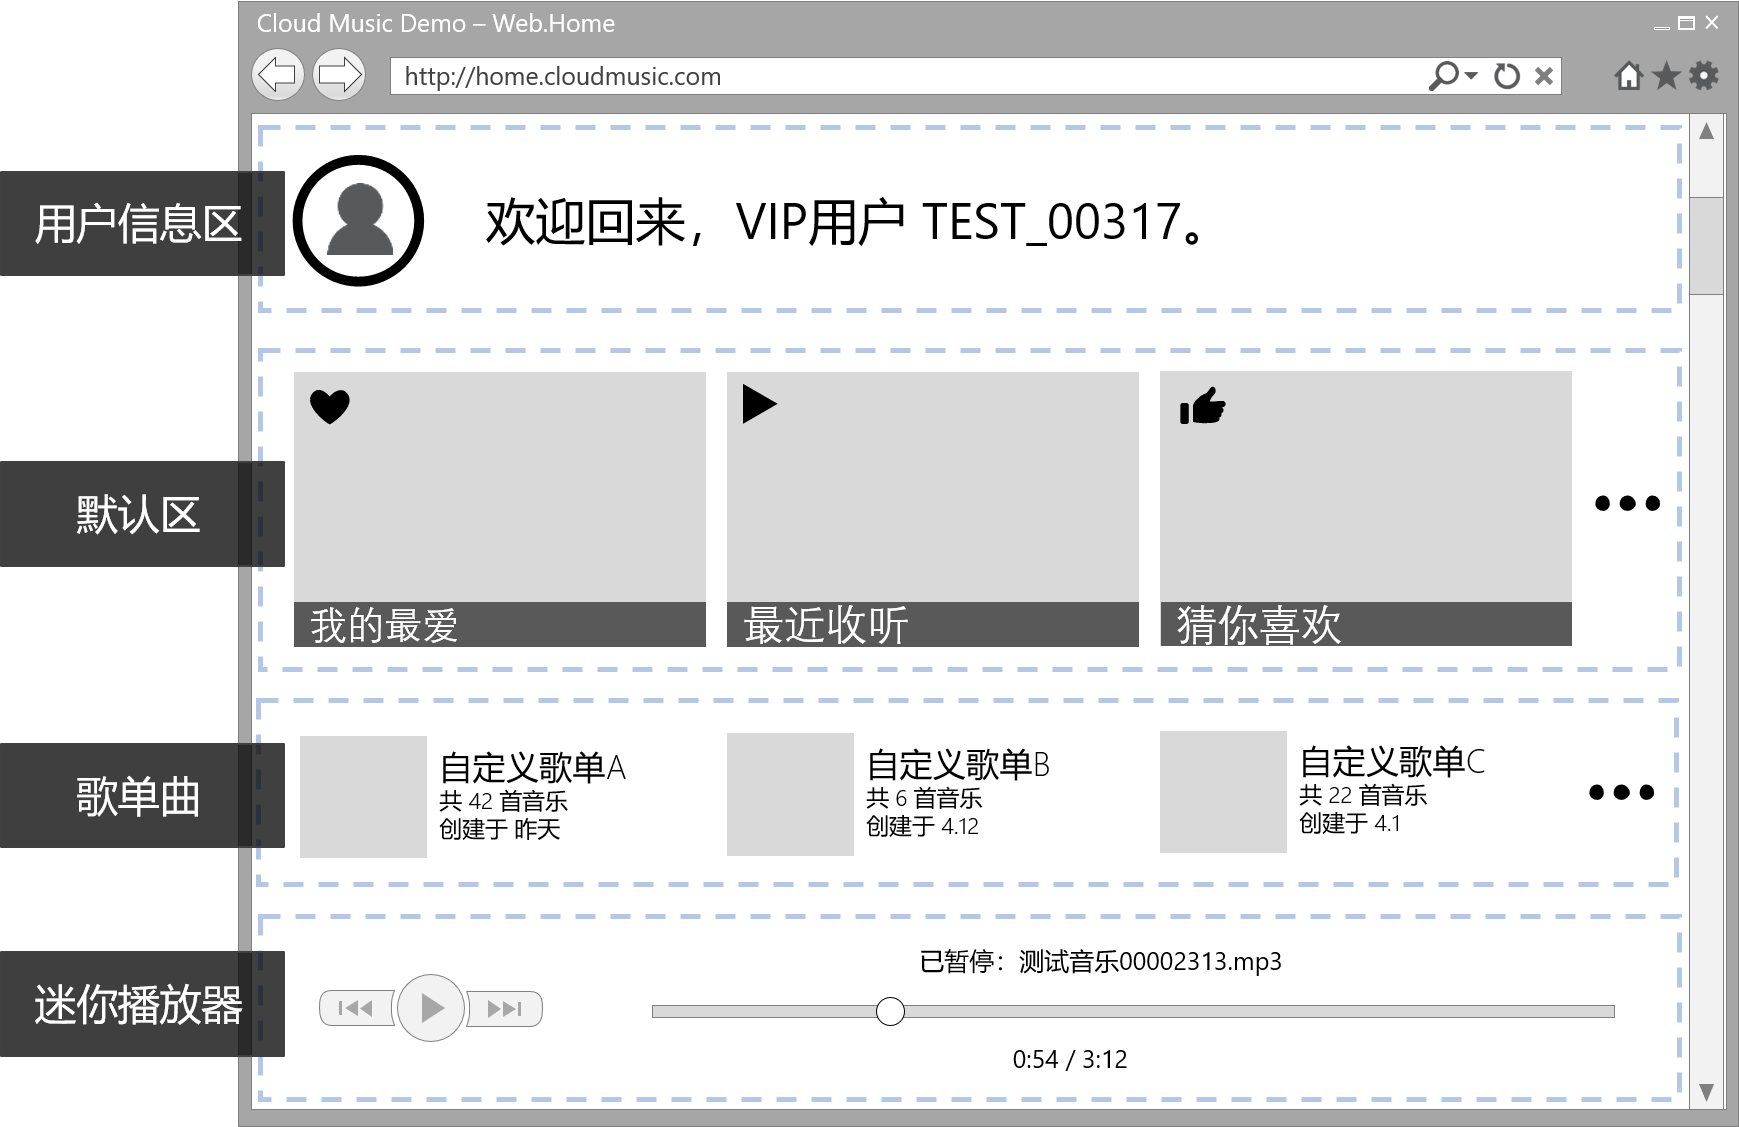
\includegraphics[width=.99\linewidth]{figures/web_home}

  \caption{  \label{fig:web_home}
  		网页客户端主页(Home Page)用户界面设计图
    }
\end{figure}

\begin{figure}[h!]
  \centering
 
  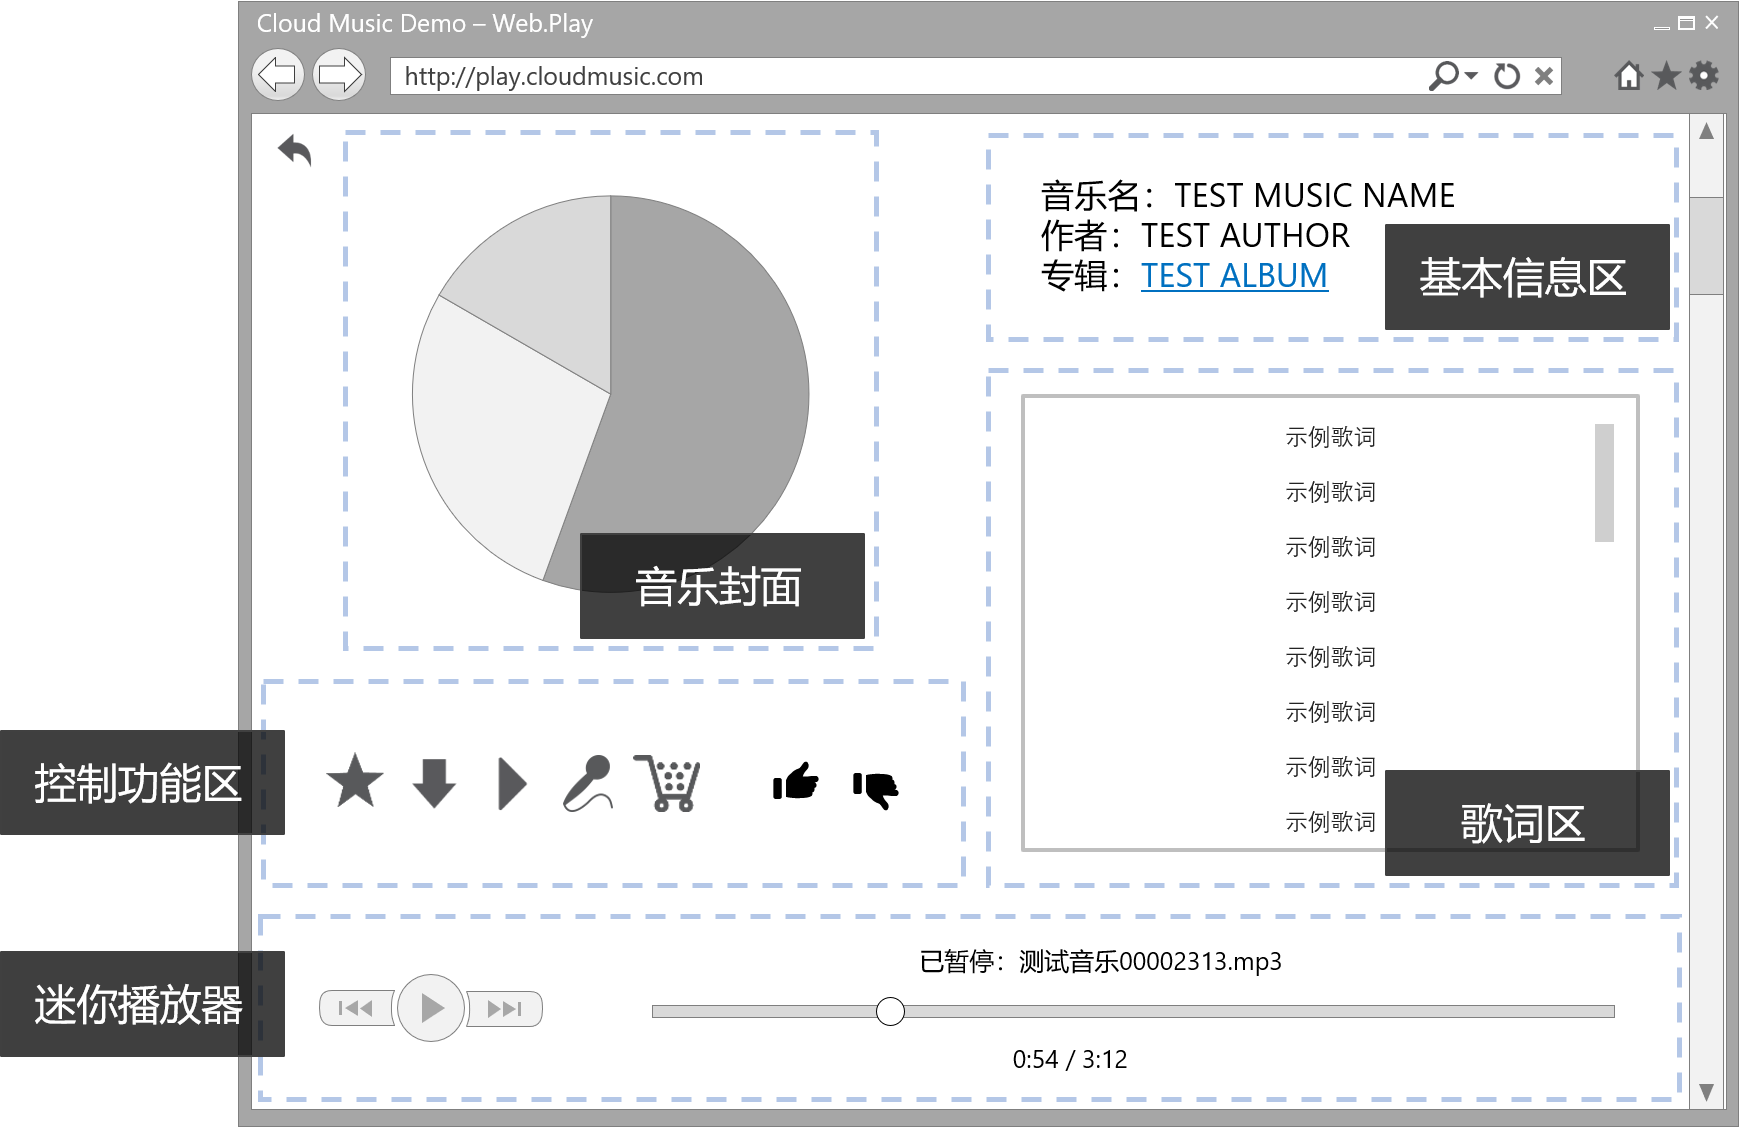
\includegraphics[width=.99\linewidth]{figures/web_music}

  \caption{ \label{fig:web_music}
  		网页客户端音乐播放界面用户界面设计图
    }
\end{figure}

\begin{figure}[h!]
  \centering

  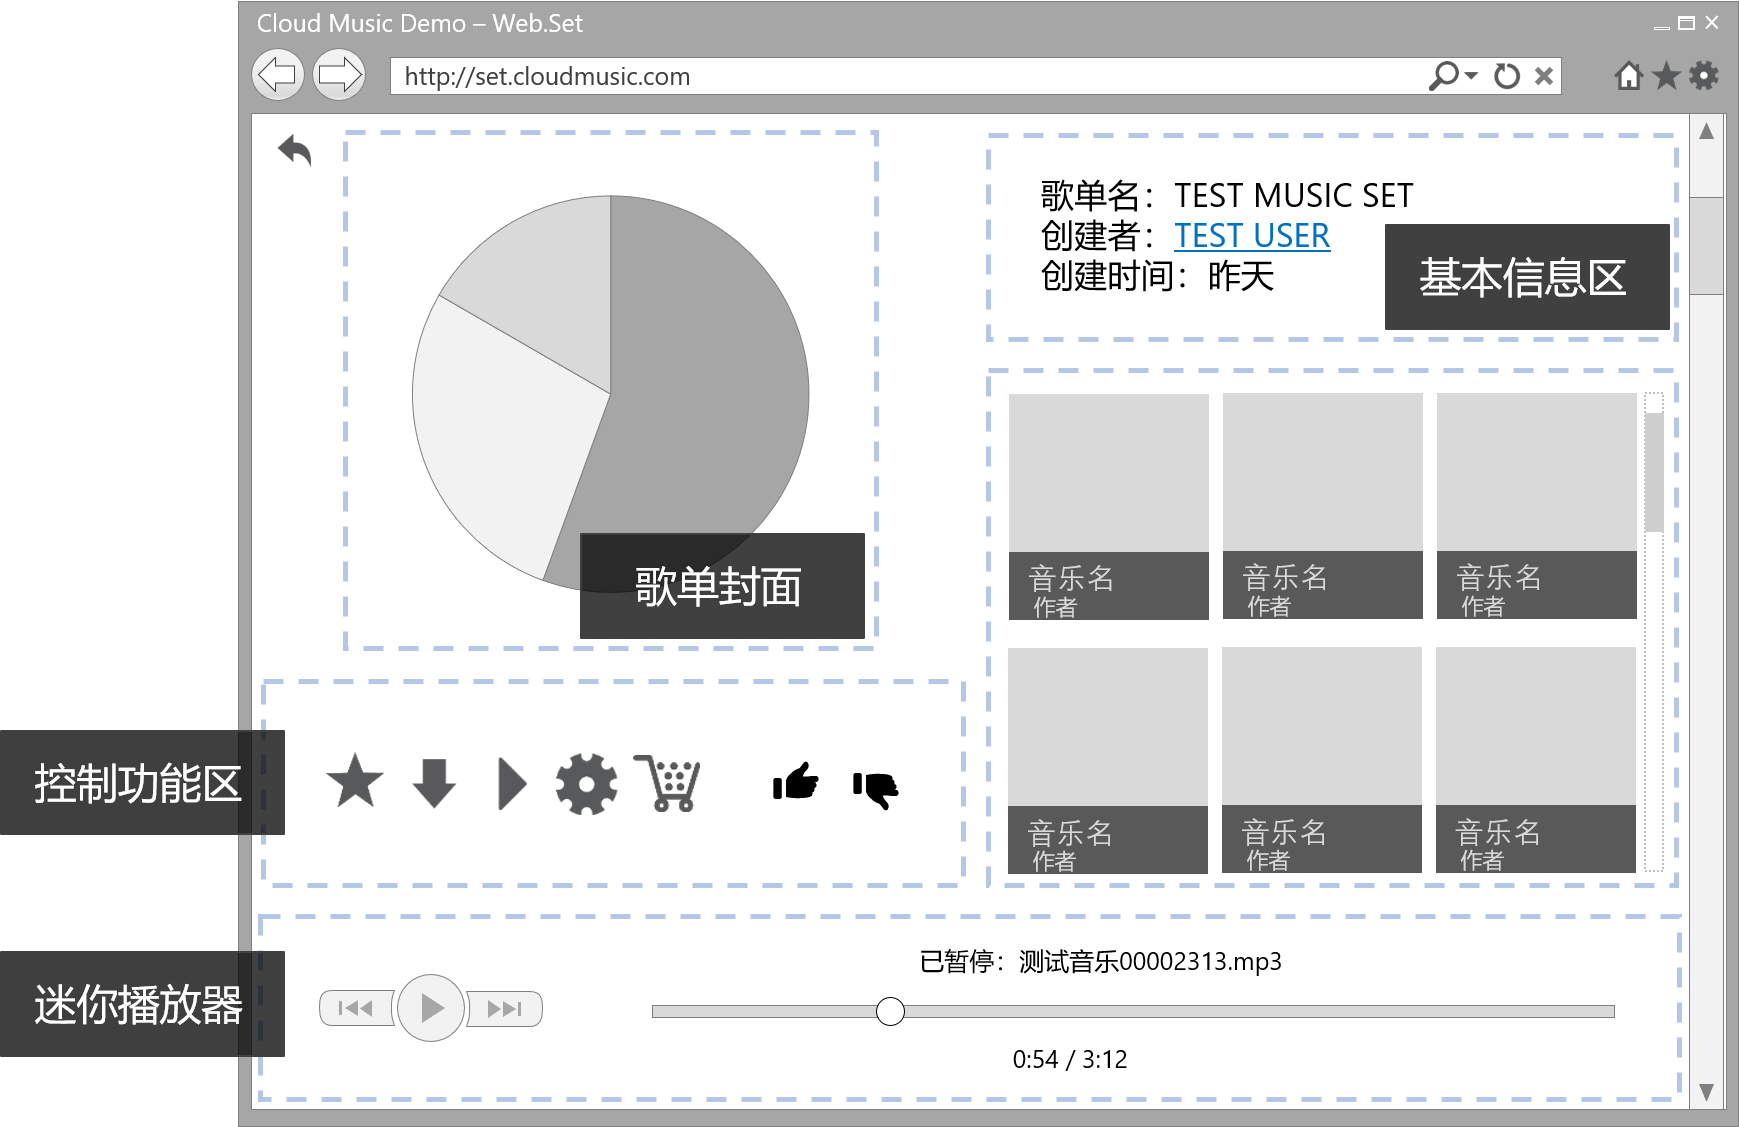
\includegraphics[width=.99\linewidth]{figures/web_collection}

  \caption{  \label{fig:web_collection}
  		网页客户端音乐集展示用户界面设计图
    }
\end{figure}
\newpage
\section{服务器端界面}
\begin{enumerate}
	\item \textbf{要求的屏幕格式}:
		服务器端仅支持在内部网页上,支持大于$800 \times 600$ 分辨率的通用网页浏览器,
		并对根据屏幕大小以及浏览器设定的屏素放大比例做自动适应;
	\item \textbf{使用方式}:
		对于管理员,我们的产品使用逻辑与一般的网页一致,
			管理员不需要主动学习便可学会使用它,
		同时,我们也会在安装后附上使用说明书,来保证管理员可以方便使用;
	\item \textbf{页面规划}: 
	\begin{itemize}
		\item 管理界面的用户界面设计,请参考图\ref{fig:sudo};
	\end{itemize}
\end{enumerate}

\begin{figure}[h!]
  \centering

  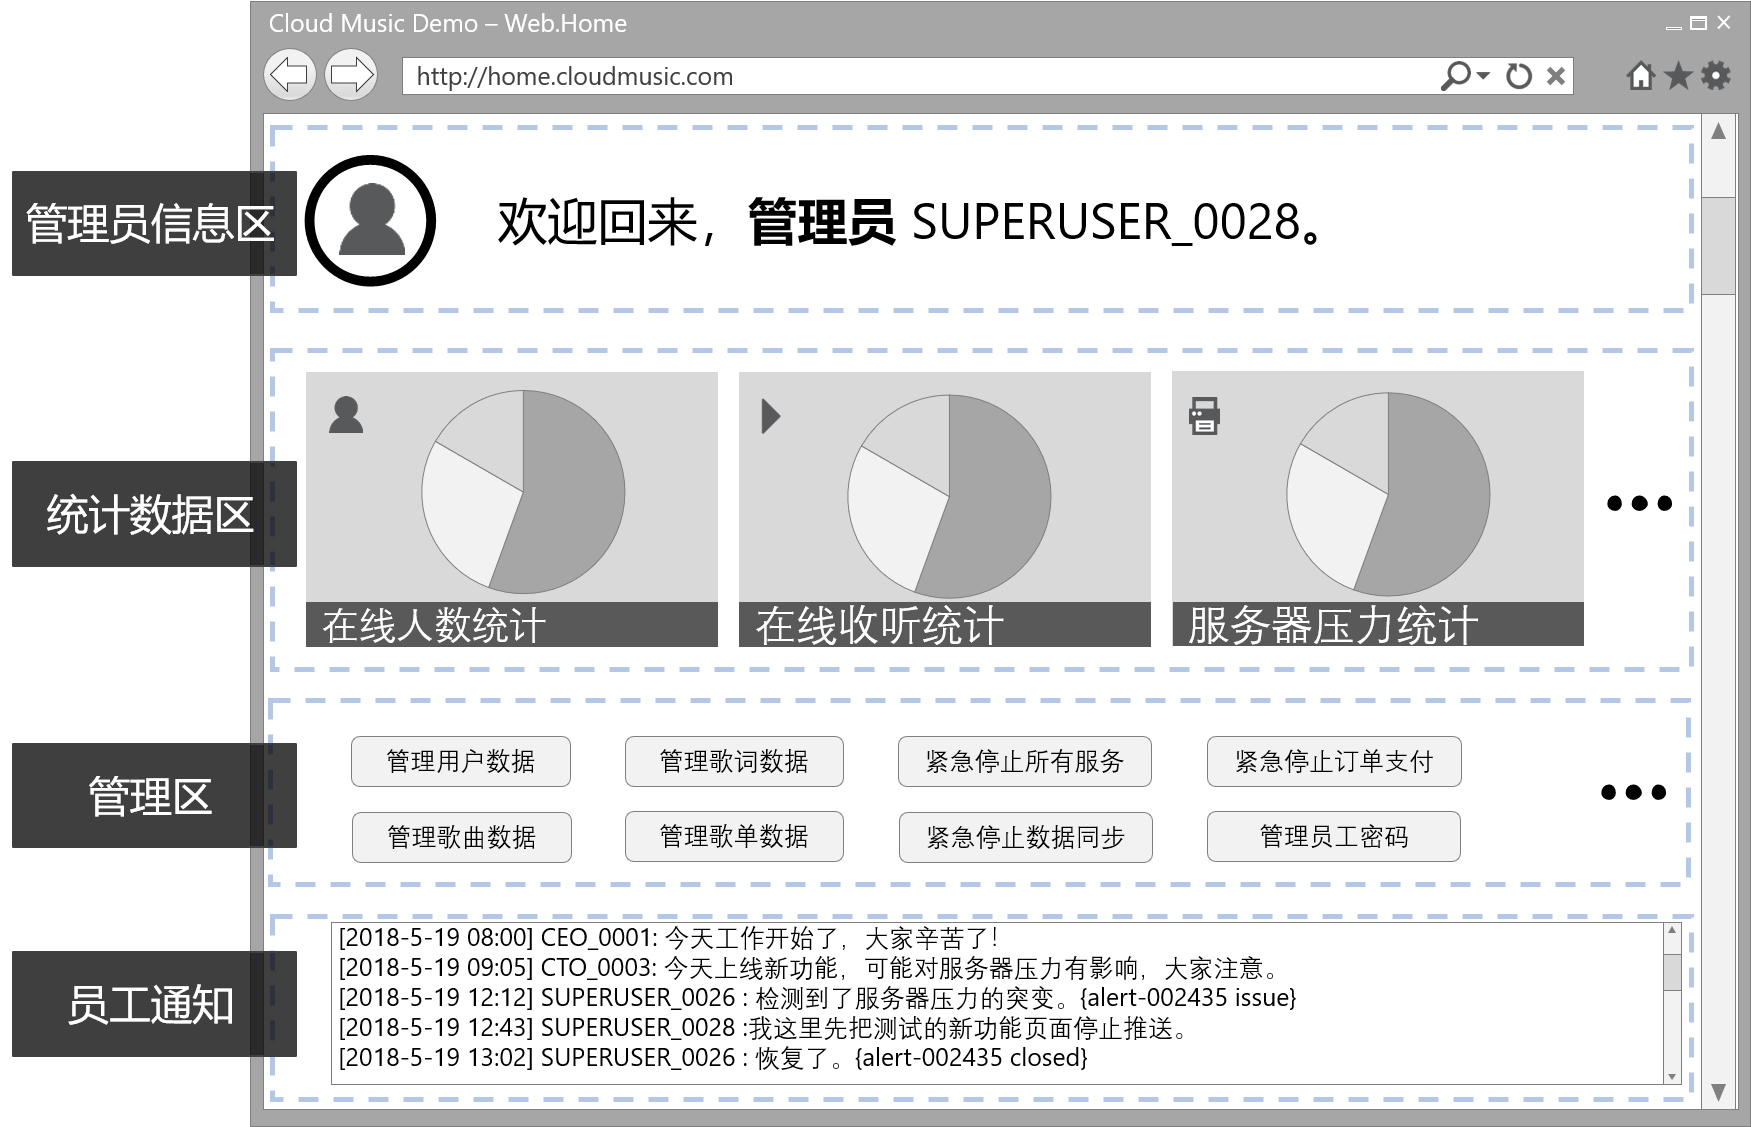
\includegraphics[width=.99\linewidth]{figures/sudo}

  \caption{  \label{fig:sudo}
  		服务端管理界面的用户界面设计图
    }
\end{figure}
\chapter{出错处理设计}
\section{数据库出错处理}

数据库备份依据数据库的不同类型与不同特征分别采取不同的备份方案。

用户等数据改变频率比较低,改变量比较小,采用事务日志备份。由于该数据库与用户登录的核心功能关联,该数据库出错时,如果有充足的服务条件,先切换到有最后一次正确的数据库的服务器上继续提供服务,等主服务器将备份数据还原之后再切换回主服务器提供服务,无需暂停服务。

评论数据等,每次改变量比较小,但改变频率极为频繁,因此采用增量和定时备份的方式备份。由于该数据库并未与核心功能关联,该数据库出错时,如果有充足的服务器条件,由备用服务器提供该服务,而不需暂停服务,主服务器仍旧提供其余部分服务,恢复备份数据后移回主服务器提供服务。

而文件数据(歌曲,图片)由于大部分情况为单个文件的变化,所以采用完全备份。该数据库出错时,如果有充足的服务器条件,可以先排查出现错误的具体功能,由备用服务器提供该功能的服务,不需暂停服务,主服务器仍旧提供其余部分服务,恢复备份数据后移回主服务器提供服务。

\section{某模块失效处理}
模块失效时,根据失效模块的功能和重要性决定处理方式。

若核心模块如储存、用户、数据库等模块失效,则应暂停整个系统的服务,由该模块的开发人员为主,在其他开发人员的支持下调整失效模块,测试完成后整体上线。

若非核心模块如图形界面、审计模块、网络请求等失效,则应先关闭失效模块提供的服务及相应接口提供的服务,其余不相关的服务维持其状态,由该模块的开发人员为主,在其他开发人员的支持下调整失效模块,测试完成后将更改的模块同时上线。
\chapter{安全保密设计}
可能的内容包括保密性、是否采取加密传输、密钥如何分发和管理等。
\chapter{维护设计}
可能的内容包括数据库的日常备份、压缩、维护等。

%\chapter{图片}
本章展示图片相关用法。

\section{示例}
\begin{figure}[ht]
\centering

\includegraphics[width=10cm]{ustc_logo_fig}
\caption{测试图片} \label{fig:figure1}
\end{figure}

\section{带图注的图}
\begin{figure}[ht]
\centering

\includegraphics[width=10cm]{ustc_logo_fig}
\caption{带图注的图片}\label{fig:noted-figure}
\note{the solid lines represent the time histogram of the spontaneous activities of an old monkey cell(gray) and a young monkey cell (black). The bin-width is 1}
\end{figure}

%\chapter{表格}

\section{A Simple Table}
\begin{table}[htbp]
\centering
\caption{这里是表的标题} \label{tab:simpletable}
\begin{tabular}{|c|c|}
    \hline
    a & b \\
    \hline
    c & d \\
    \hline
\end{tabular}
\note{这里是表的注释}
\end{table}

\section{长表格}
\begin{longtable}{ccc}
% 首页表头
\caption[长表格演示]{长表格演示} \label{tab:longtable} \\
\toprule[1.5pt]
名称  & 说明 & 备注\\
\midrule[1pt]
\endfirsthead
% 续页表头
\caption[]{长表格演示(续)} \\
\toprule[1.5pt]
名称  & 说明 & 备注 \\
\midrule[1pt]
\endhead
% 首页表尾
\hline
\multicolumn{3}{r}{\small 续下页}
\endfoot
% 续页表尾
\bottomrule[1.5pt]
\endlastfoot

AAAAAAAAAAAA   &   BBBBBBBBBBB   &   CCCCCCCCCCCCCC   \\
AAAAAAAAAAAA   &   BBBBBBBBBBB   &   CCCCCCCCCCCCCC   \\
AAAAAAAAAAAA   &   BBBBBBBBBBB   &   CCCCCCCCCCCCCC   \\
AAAAAAAAAAAA   &   BBBBBBBBBBB   &   CCCCCCCCCCCCCC   \\
AAAAAAAAAAAA   &   BBBBBBBBBBB   &   CCCCCCCCCCCCCC   \\
AAAAAAAAAAAA   &   BBBBBBBBBBB   &   CCCCCCCCCCCCCC   \\
AAAAAAAAAAAA   &   BBBBBBBBBBB   &   CCCCCCCCCCCCCC   \\
AAAAAAAAAAAA   &   BBBBBBBBBBB   &   CCCCCCCCCCCCCC   \\
AAAAAAAAAAAA   &   BBBBBBBBBBB   &   CCCCCCCCCCCCCC   \\
AAAAAAAAAAAA   &   BBBBBBBBBBB   &   CCCCCCCCCCCCCC   \\
AAAAAAAAAAAA   &   BBBBBBBBBBB   &   CCCCCCCCCCCCCC   \\
AAAAAAAAAAAA   &   BBBBBBBBBBB   &   CCCCCCCCCCCCCC   \\
AAAAAAAAAAAA   &   BBBBBBBBBBB   &   CCCCCCCCCCCCCC   \\
AAAAAAAAAAAA   &   BBBBBBBBBBB   &   CCCCCCCCCCCCCC   \\
AAAAAAAAAAAA   &   BBBBBBBBBBB   &   CCCCCCCCCCCCCC   \\
AAAAAAAAAAAA   &   BBBBBBBBBBB   &   CCCCCCCCCCCCCC   \\
AAAAAAAAAAAA   &   BBBBBBBBBBB   &   CCCCCCCCCCCCCC   \\
AAAAAAAAAAAA   &   BBBBBBBBBBB   &   CCCCCCCCCCCCCC   \\
AAAAAAAAAAAA   &   BBBBBBBBBBB   &   CCCCCCCCCCCCCC   \\
AAAAAAAAAAAA   &   BBBBBBBBBBB   &   CCCCCCCCCCCCCC   \\
AAAAAAAAAAAA   &   BBBBBBBBBBB   &   CCCCCCCCCCCCCC   \\
AAAAAAAAAAAA   &   BBBBBBBBBBB   &   CCCCCCCCCCCCCC   \\
AAAAAAAAAAAA   &   BBBBBBBBBBB   &   CCCCCCCCCCCCCC   \\
AAAAAAAAAAAA   &   BBBBBBBBBBB   &   CCCCCCCCCCCCCC   \\
AAAAAAAAAAAA   &   BBBBBBBBBBB   &   CCCCCCCCCCCCCC   \\
AAAAAAAAAAAA   &   BBBBBBBBBBB   &   CCCCCCCCCCCCCC   \\
AAAAAAAAAAAA   &   BBBBBBBBBBB   &   CCCCCCCCCCCCCC   \\
AAAAAAAAAAAA   &   BBBBBBBBBBB   &   CCCCCCCCCCCCCC   \\
AAAAAAAAAAAA   &   BBBBBBBBBBB   &   CCCCCCCCCCCCCC   \\
AAAAAAAAAAAA   &   BBBBBBBBBBB   &   CCCCCCCCCCCCCC   \\
AAAAAAAAAAAA   &   BBBBBBBBBBB   &   CCCCCCCCCCCCCC   \\
AAAAAAAAAAAA   &   BBBBBBBBBBB   &   CCCCCCCCCCCCCC   \\
AAAAAAAAAAAA   &   BBBBBBBBBBB   &   CCCCCCCCCCCCCC   \\
AAAAAAAAAAAA   &   BBBBBBBBBBB   &   CCCCCCCCCCCCCC   \\
AAAAAAAAAAAA   &   BBBBBBBBBBB   &   CCCCCCCCCCCCCC   \\
AAAAAAAAAAAA   &   BBBBBBBBBBB   &   CCCCCCCCCCCCCC   \\
\end{longtable}

%\chapter{算法环境}
模板中使用 \texttt{algorithm2e} 宏包实现算法环境。关于该宏包的具体用法,
请阅读宏包的官方文档。

\begin{algorithm}[htbp]
\SetAlgoLined
\KwData{this text}
\KwResult{how to write algorithm with \LaTeX2e }

initialization\;
\While{not at end of this document}{
    read current\;
    \eIf{understand}{
        go to next section\;
        current section becomes this one\;
    }{
        go back to the beginning of current section\;
    }
}
\caption{算法示例1}
\label{algo:algorithm1}
\end{algorithm}

\IncMargin{1em}
\begin{algorithm}
\SetKwData{Left}{left}\SetKwData{This}{this}\SetKwData{Up}{up}
\SetKwFunction{Union}{Union}\SetKwFunction{FindCompress}{FindCompress}
\SetKwInOut{Input}{input}\SetKwInOut{Output}{output}

\Input{A bitmap $Im$ of size $w\times l$}
\Output{A partition of the bitmap}
\BlankLine
\emph{special treatment of the first line}\;
\For{$i\leftarrow 2$ \KwTo $l$}{
    \emph{special treatment of the first element of line $i$}\;
    \For{$j\leftarrow 2$ \KwTo $w$}{\label{forins}
        \Left$\leftarrow$ \FindCompress{$Im[i,j-1]$}\;
        \Up$\leftarrow$ \FindCompress{$Im[i-1,]$}\;
        \This$\leftarrow$ \FindCompress{$Im[i,j]$}\;
        \If(\tcp*[h]{O(\Left,\This)==1}){\Left compatible with \This}{\label{lt}
            \lIf{\Left $<$ \This}{\Union{\Left,\This}}
            \lElse{\Union{\This,\Left}}
        }
        \If(\tcp*[f]{O(\Up,\This)==1}){\Up compatible with \This}{\label{ut}
        \lIf{\Up $<$ \This}{\Union{\Up,\This}}
        \tcp{\This is put under \Up to keep tree as flat as possible}\label{cmt}
        \lElse{\Union{\This,\Up}}\tcp*[h]{\This linked to \Up}\label{lelse}
        }
    }
    \lForEach{element $e$ of the line $i$}{\FindCompress{p}}
}
\caption{算法示例2}\label{algo_disjdecomp}
\label{alog:algorithm2}
\end{algorithm}\DecMargin{1em}

%\chapter{代码环境}
模板中使用 \texttt{listings} 宏包实现代码环境。详细用法见宏包的官方说明文档。

以下是代码示例,可以在文中任意位置引用\autoref{first-code} 。
\begin{lstlisting}[language=C, caption=示例代码, label={code:first-code}]
#include <stdio.h>

int main( )
{
    printf("hello, world\n");
    return 0;
}
\end{lstlisting}

%\chapter{引用文献标注}

\section{著者-出版年制标注法}

\noindent
\verb|\citestyle{ustcauthoryear}|
\citestyle{ustcauthoryear}

\noindent
\begin{tabular}{l@{\quad$\Rightarrow$\quad}l}
  \verb|\cite{knuth86a}| & \cite{knuth86a}\\
  \verb|\citet{knuth86a}| & \citet{knuth86a}\\
  \verb|\citet[chap.~2]{knuth86a}| & \citet[chap.~2]{knuth86a}\\[0.5ex]
  \verb|\citep{knuth86a}| & \citep{knuth86a}\\
  \verb|\citep[chap.~2]{knuth86a}| & \citep[chap.~2]{knuth86a}\\
  \verb|\citep[see][]{knuth86a}| & \citep[see][]{knuth86a}\\
  \verb|\citep[see][chap.~2]{knuth86a}| & \citep[see][chap.~2]{knuth86a}\\[0.5ex]
  \verb|\citet*{knuth86a}| & \citet*{knuth86a}\\
  \verb|\citep*{knuth86a}| & \citep*{knuth86a}\\
\end{tabular}

\noindent
\begin{tabular}{l@{\quad$\Rightarrow$\quad}l}
  \verb|\citet{knuth86a,tlc2}| & \citet{knuth86a,tlc2}\\
  \verb|\citep{knuth86a,tlc2}| & \citep{knuth86a,tlc2}\\
  \verb|\cite{knuth86a,knuth84}| & \cite{knuth86a,knuth84}\\
  \verb|\citet{knuth86a,knuth84}| & \citet{knuth86a,knuth84}\\
  \verb|\citep{knuth86a,knuth84}| & \citep{knuth86a,knuth84}\\
\end{tabular}

\section{顺序编码制标注法}

\noindent
\verb|\citestyle{ustcnumerical}|
\citestyle{ustcnumerical}

\noindent
\begin{tabular}{l@{\quad$\Rightarrow$\quad}l}
  \verb|\cite{knuth86a}| & \cite{knuth86a}\\
  \verb|\citet{knuth86a}| & \citet{knuth86a}\\
  \verb|\citet[chap.~2]{knuth86a}| & \citet[chap.~2]{knuth86a}\\[0.5ex]
  \verb|\citep{knuth86a}| & \citep{knuth86a}\\
  \verb|\citep[chap.~2]{knuth86a}| & \citep[chap.~2]{knuth86a}\\
  \verb|\citep[see][]{knuth86a}| & \citep[see][]{knuth86a}\\
  \verb|\citep[see][chap.~2]{knuth86a}| & \citep[see][chap.~2]{knuth86a}\\[0.5ex]
  \verb|\citet*{knuth86a}| & \citet*{knuth86a}\\
  \verb|\citep*{knuth86a}| & \citep*{knuth86a}\\
\end{tabular}

\noindent
\begin{tabular}{l@{\quad$\Rightarrow$\quad}l}
  \verb|\citet{knuth86a,tlc2}| & \citet{knuth86a,tlc2}\\
  \verb|\citep{knuth86a,tlc2}| & \citep{knuth86a,tlc2}\\
  \verb|\cite{knuth86a,knuth84}| & \cite{knuth86a,knuth84}\\
  \verb|\citet{knuth86a,knuth84}| & \citet{knuth86a,knuth84}\\
  \verb|\citep{knuth86a,knuth84}| & \citep{knuth86a,knuth84}\\
  \verb|\cite{knuth86a,knuth84,tlc2}| & \cite{knuth86a,knuth84,tlc2}\\
\end{tabular}

\section{其他形式的标注}

\noindent
\begin{tabular}{l@{\quad$\Rightarrow$\quad}l}
  \verb|\citealt{tlc2}| & \citealt{tlc2}\\
  \verb|\citealt*{tlc2}| & \citealt*{tlc2}\\
  \verb|\citealp{tlc2}| & \citealp{tlc2}\\
  \verb|\citealp*{tlc2}| & \citealp*{tlc2}\\
  \verb|\citealp{tlc2,knuth86a}| & \citealp{tlc2,knuth86a}\\
  \verb|\citealp[pg.~32]{tlc2}| & \citealp[pg.~32]{tlc2}\\
  \verb|\citenum{tlc2}| & \citenum{tlc2}\\
  \verb|\citetext{priv.\ comm.}| & \citetext{priv.\ comm.}\\
\end{tabular}

\noindent
\begin{tabular}{l@{\quad$\Rightarrow$\quad}l}
  \verb|\citeauthor{tlc2}| & \citeauthor{tlc2}\\
  \verb|\citeauthor*{tlc2}| & \citeauthor*{tlc2}\\
  \verb|\citeyear{tlc2}| & \citeyear{tlc2}\\
  \verb|\citeyearpar{tlc2}| & \citeyearpar{tlc2}\\
\end{tabular}

\bibliography{bib/tex}


\end{document}
